\documentclass[aspectratio=169, 10pt]{beamer}

% ==============================================================================
% THEME & STYLING CONFIGURATION - MANUAL DE IDENTIDADE VISUAL CIn-UFPE (Ago. 2020)
% ==============================================================================
\usetheme{Madrid}
\useinnertheme{rectangles}
\setbeamertemplate{navigation symbols}{} % Remove default navigation buttons

% ------------------------------------------------------------------------------
% PALETA DE CORES INSTITUCIONAIS (Página 11 do Manual de Identidade Visual)
% ------------------------------------------------------------------------------
% 1. Vermelho Primário (Pantone 1795 C)
\definecolor{cinRed}{RGB}{219, 30, 47}         % #DB1E2F - Cor Primária Institucional
% 2. Vermelho Escuro (Pantone 200 C)
\definecolor{cinDarkRed}{RGB}{175, 4, 33}      % #AF0421 - Secundária / Profundidade / Destaque
% 3. Preto Institucional (Pantone 419 C)
\definecolor{cinBlack}{RGB}{35, 31, 32}        % #231F20 - Tipografia / Títulos / Contraste
% 4. Cinza Claro (Pantone 664 C)
\definecolor{cinLightGray}{RGB}{224, 225, 224} % #E0E1E0 - Fundos de Blocos / Separações
% Cores Neutras de Apoio
\definecolor{cinOffWhite}{RGB}{250, 250, 250}  % #FAFAFA - Fundo limpo
\definecolor{cinMidGray}{RGB}{100, 100, 100}   % #646464 - Texto secundário
\definecolor{cinGold}{RGB}{204, 153, 0}        % #CC9900 - Destaque métrico / Alerta

% Beamer Color Mappings com a Paleta Oficial CIn
\setbeamercolor{palette primary}{bg=cinRed, fg=white}
\setbeamercolor{palette secondary}{bg=cinDarkRed, fg=white}
\setbeamercolor{palette tertiary}{bg=cinBlack, fg=white}
\setbeamercolor{structure}{fg=cinRed}
\setbeamercolor{titlelike}{parent=structure, fg=cinDarkRed}
\setbeamercolor{frametitle}{bg=cinRed, fg=white}
\setbeamercolor{frametitle right}{bg=cinDarkRed}

% Block Colors (Harmonizados com o Manual: Vermelho CIn, Vermelho Escuro e Cinza Claro)
\setbeamercolor{block title}{bg=cinRed, fg=white}
\setbeamercolor{block body}{bg=cinLightGray!35, fg=cinBlack}
\setbeamercolor{block title example}{bg=cinDarkRed, fg=white}
\setbeamercolor{block body example}{bg=cinLightGray!25, fg=cinBlack}
\setbeamercolor{block title alerted}{bg=cinBlack, fg=white}
\setbeamercolor{block body alerted}{bg=cinLightGray!30, fg=cinDarkRed}

% Itemize and Enumerate
\setbeamercolor{item}{fg=cinRed}
\setbeamercolor{subitem}{fg=cinDarkRed}
\setbeamertemplate{itemize item}{\scriptsize\raise1pt\hbox{\donotcoloroutermaths$\blacksquare$}}
\setbeamertemplate{itemize subitem}{\tiny\raise1pt\hbox{\donotcoloroutermaths$\blacktriangleright$}}

% Custom Footline com Identidade CIn-UFPE
\setbeamertemplate{footline}{
  \leavevmode%
  \hbox{%
  \begin{beamercolorbox}[wd=.333333\paperwidth,ht=2.4ex,dp=1.1ex,left,leftskip=2ex]{author in head/foot}%
    \usebeamerfont{author in head/foot}\textbf{Fagner Candido} \textbar\ CIn--UFPE
  \end{beamercolorbox}%
  \begin{beamercolorbox}[wd=.416667\paperwidth,ht=2.4ex,dp=1.1ex,center]{title in head/foot}%
    \usebeamerfont{title in head/foot}\textbf{PANOPTES:} Kubernetes Observability
  \end{beamercolorbox}%
  \begin{beamercolorbox}[wd=.25\paperwidth,ht=2.4ex,dp=1.1ex,right,rightskip=2ex]{date in head/foot}%
    \usebeamerfont{date in head/foot}Qualificação \hfill \insertframenumber{} / \inserttotalframenumber
  \end{beamercolorbox}}%
  \vskip0pt%
}

% ==============================================================================
% PACKAGES
% ==============================================================================
\usepackage[utf8]{inputenc}
\usepackage[T1]{fontenc}
\usepackage{lmodern}
\usepackage{booktabs}
\usepackage{tabularx}
\usepackage{multirow}
\usepackage{colortbl}
\usepackage{amsmath,amssymb}
\usepackage{graphicx}
\graphicspath{{.}{./}{images/}{../images/}}
\usepackage{tikz}
\usetikzlibrary{arrows.meta, positioning, shapes.geometric, calc, fit, backgrounds}

% ==============================================================================
% METADATA
% ==============================================================================
\title[\textbf{PANOPTES:} Kubernetes Observability]{\textbf{PANOPTES:} An Open-Source Reference Architecture for Observability in Kubernetes Ecosystems}
\subtitle{Exame de Qualificação de Doutorado / Doctoral Qualification Defense}

\author[\textbf{Fagner Candido}]{
  \textbf{Candidato:} Fagner Fernandes Candido da Silva\\[1ex]
  \small \textbf{Orientador:} Prof. Dr. Vinícius Cardoso Garcia\\
  \small \textbf{Coorientador:} Prof. Dr. Jackson Raniel Florêncio da Silva
}

\institute[CIn--UFPE]{
  \inst{} Centro de Informática (CIn) \\
  Universidade Federal de Pernambuco (UFPE) \\
  Programa de Pós-Graduação em Ciência da Computação (PPGCC) \\
  \textit{Área: Engenharia de Software e Linguagens de Programação}
}

\date{2026}

% ==============================================================================
% DOCUMENT BODY
% ==============================================================================
\begin{document}

% ------------------------------------------------------------------------------
% Slide 1: Title Slide
% ------------------------------------------------------------------------------
\begin{frame}[plain]
  \titlepage
  \vspace{-3ex}
  \begin{center}
    
\includegraphics[height=1.1cm]{HC.png}
  \end{center}
\end{frame}

% ------------------------------------------------------------------------------
% Slide 2: Outline
% ------------------------------------------------------------------------------
\begin{frame}{Agenda da Apresentação}
  \tableofcontents
\end{frame}

% ==============================================================================
% SECTION 1: CONTEXT, PROBLEM & MOTIVATION
% ==============================================================================
\section{Contexto, Motivação \& Problema de Pesquisa}

\begin{frame}{O Paradigma Cloud-Native \& a Complexidade do Kubernetes}
  \begin{columns}[T]
    \begin{column}{0.58\textwidth}
      \begin{block}{A Transição Arquitetural}
        \small
        \begin{itemize}
          \item \textbf{Monólitos $\rightarrow$ Microsserviços:} Desacoplamento funcional, pipelines elásticos e deploys poliglota contínuos.
          \item \textbf{Kubernetes (K8s):} Orquestração autônoma de contêineres e auto-scaling como padrão de fato da indústria.
        \end{itemize}
      \end{block}
      \vspace{-0.5ex}
      \begin{alertblock}{O Desafio Operacional Emergente}
        \small
        \begin{itemize}
          \item \textbf{Efemeridade Extrema:} Pods surgem e terminam dinamicamente; IPs perdem relevância diagnóstica estática.
          \item \textbf{Explosão Telemétrica:} Volume e velocidade massivos de métricas, logs e traces distribuídos.
          \item \textbf{Falhas Latentes (\textit{Unknown Unknowns}):} Degradações assíncronas em cascata que não disparam limites de CPU ou memória.
        \end{itemize}
      \end{alertblock}
    \end{column}
    
    \begin{column}{0.38\textwidth}
      \begin{exampleblock}{Dados da Indústria (CNCF)}
        \footnotesize \centering
        \textbf{$> 84\%$} utilizam Kubernetes em produção.\\[1ex]
        \textbf{Maior Desafio:}\\
        \textit{"Complexidade de troubleshooting e aumento de MTTR por silos telemétricos."}
      \end{exampleblock}
      \vspace{0.5ex}
      \centering
      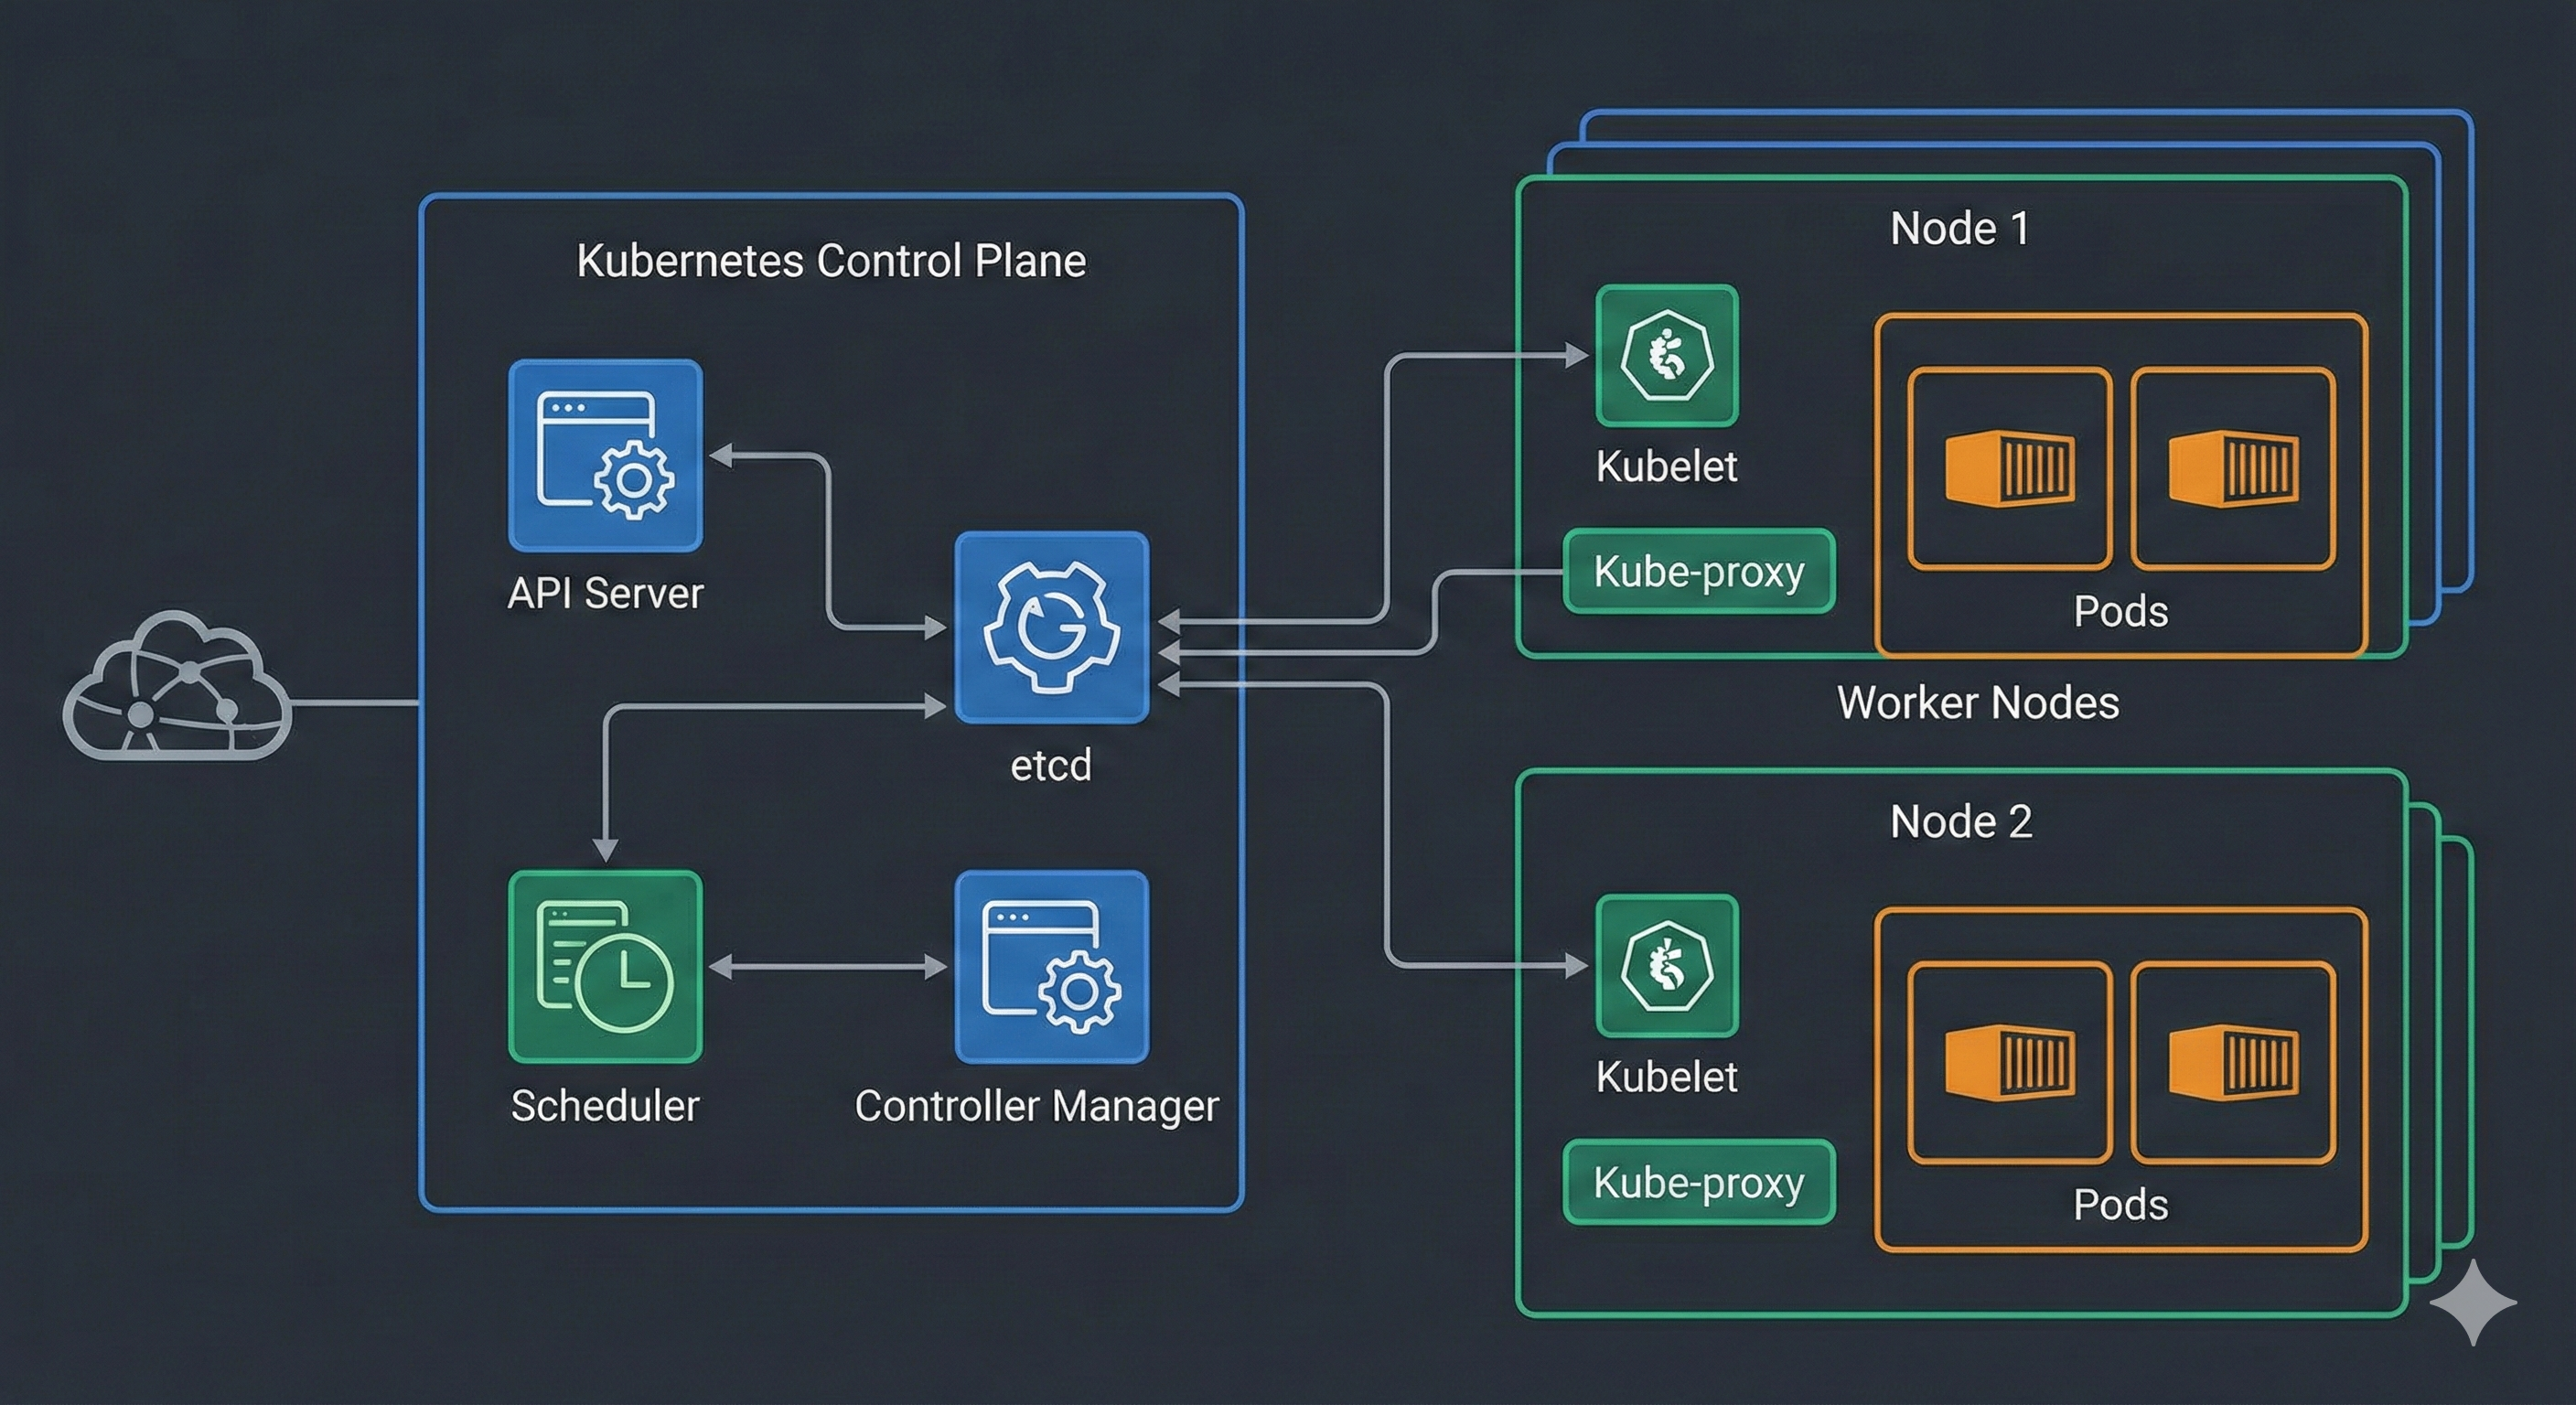
\includegraphics[height=0.36\textheight, keepaspectratio]{cloud-computing/k8s-architecture.png}
    \end{column}
  \end{columns}
\end{frame}

\begin{frame}{Fundamentação Teórica: O Conceito Canônico de Kalman}
  \begin{columns}[T]
    \begin{column}{0.48\textwidth}
      \begin{block}{Conceito Canônico de Observabilidade (Kalman, 1959)}
        \small \textit{"Um sistema dinâmico é dito \textbf{observável} se o seu estado interno $x(t)$ pode ser integralmente determinado em tempo finito a partir exclusivamente do conhecimento de suas saídas mensuráveis $y(t)$ e entradas conhecidas $u(t)$."}
      \end{block}
      \vspace{0.8ex}
      \begin{alertblock}{O Desafio em Sistemas Distribuídos}
        \small
        \begin{itemize}
          \item Em orquestradores de microsserviços, falhas latentes ocorrem sem violação de limites estáticos de CPU/RAM (\textit{known unknowns});
          \item A determinação da causa-raiz exige reconstruir a dinâmica interna a partir de telemetria rica e correlacionada (\textit{unknown unknowns}).
        \end{itemize}
      \end{alertblock}
    \end{column}
    
    \begin{column}{0.50\textwidth}
      \centering
      \resizebox{0.94\linewidth}{!}{%
      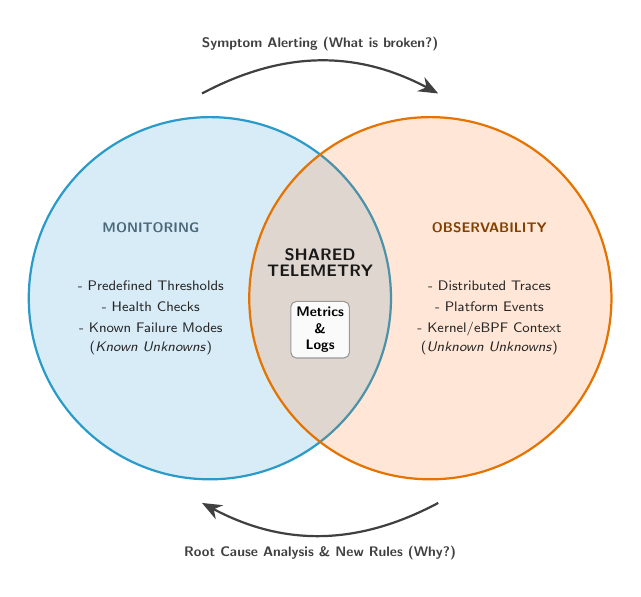
\begin{tikzpicture}[
          font=\sffamily,
          circle_node/.style={circle, minimum size=4.6cm, fill opacity=0.16, text opacity=1, draw, thick},
          label_title/.style={font=\sffamily\bfseries\tiny, align=center},
          bullet_text/.style={font=\sffamily\tiny, align=center, text width=2.0cm},
          arrow_style/.style={-{Stealth[length=2.5mm, width=2mm]}, thick, draw=darkgray}
      ]

          % Circles (Radius = 2.3cm; Centers at -1.4 and 1.4 -> Intersection width = 1.8cm)
          \node[circle_node, fill=cyan!70!blue, draw=cyan!80!black] (mon) at (-1.4, 0) {};
          \node[circle_node, fill=orange!80!red, draw=orange!90!black] (obs) at (1.4, 0) {};

          % Left Side: Monitoring Specific
          \node[label_title, text=cyan!40!black] at (-2.15, 0.9) {MONITORING};
          \node[bullet_text, text=black!85] at (-2.15, -0.25) {
              \fontsize{5.5}{6.5}\selectfont
              - Predefined Thresholds\\[1pt]
              - Health Checks\\[1pt]
              - Known Failure Modes\\[1pt]
              (\textit{Known Unknowns})
          };

          % Right Side: Observability Specific
          \node[label_title, text=orange!50!black] at (2.15, 0.9) {OBSERVABILITY};
          \node[bullet_text, text=black!85] at (2.15, -0.25) {
              \fontsize{5.5}{6.5}\selectfont
              - Distributed Traces\\[1pt]
              - Platform Events\\[1pt]
              - Kernel/eBPF Context\\[1pt]
              (\textit{Unknown Unknowns})
          };
          % Intersection: Shared Foundation
          \node[font=\sffamily\bfseries\fontsize{6}{7}\selectfont, align=center, text=black!90] at (0, 0.45) {SHARED\\[-1pt]TELEMETRY};
          \node[font=\sffamily\bfseries\fontsize{5}{6}\selectfont, align=center, fill=white, fill opacity=0.9, text opacity=1, inner sep=2pt, rounded corners=2pt, draw=black!40] at (0, -0.40) {\textbf{Metrics}\\ \& \\\textbf{Logs}};

          % Top and Bottom Workflow Arrows
          \draw[arrow_style] (-1.5, 2.6) to[bend left=28] node[midway, above, font=\sffamily\bfseries\fontsize{5}{6}\selectfont, text=darkgray] {Symptom Alerting (What is broken?)} (1.5, 2.6);
          \draw[arrow_style] (1.5, -2.6) to[bend left=28] node[midway, below, font=\sffamily\bfseries\fontsize{5}{6}\selectfont, text=darkgray] {Root Cause Analysis \& New Rules (Why?)} (-1.5, -2.6);

      \end{tikzpicture}%
      }
    \end{column}
  \end{columns}
\end{frame}

\begin{frame}{Mapeamento da Observabilidade para Sistemas Cloud-Native}
  \begin{columns}[T]
    \begin{column}{0.49\textwidth}
      \begin{block}{Mapeamento das Variáveis de Estado}
        \small
        \begin{itemize}
          \item \textbf{Estado Interno $x(t)$:} Saúde dos nós, esgotamento de conexões, buffers de memória, saturação de threads e contenção de I/O.
          \item \textbf{Entradas Conhecidas $u(t)$:} Requisições de clientes, eventos do kube-scheduler, escalonamento horizontal e perturbações de infraestrutura.
          \item \textbf{Saídas Mensuráveis $y(t)$:} A tupla telemétrica quadridimensional:
            \begin{equation*}
              \mathcal{O} = \{ \text{Métricas}, \text{Logs}, \text{Traces}, \text{Eventos} \}
            \end{equation*}
        \end{itemize}
      \end{block}
    \end{column}
    
    \begin{column}{0.49\textwidth}
      \begin{exampleblock}{Dualidade Controlabilidade-Observabilidade}
        \small
        \begin{itemize}
          \item \textbf{Teorema de Controle Estendido:} Um sistema só pode ser controlado ou autocurado na medida em que seus estados forem formalmente observáveis.
          \item \textbf{Falha do Self-Healing Cego:} Mecanismos de AIOps ou orquestradores que agem sobre dados incompletos provocam oscilações e degradações destrutivas.
        \end{itemize}
      \end{exampleblock}
      \vspace{0.8ex}
      \begin{alertblock}{Objetivo do PANOPTES}
        \small
        Correlacionar semanticamente a tupla $\mathcal{O}$ em tempo real para permitir reconstrução causal fidedigna de $x(t)$.
      \end{alertblock}
    \end{column}
  \end{columns}
\end{frame}

\begin{frame}{O Diagnóstico Padrão do Kubernetes e suas Limitações}
  \begin{columns}[T]
    \begin{column}{0.55\textwidth}
      \begin{block}{Inspeção Nativa via CLI (Vanilla K8s)}
        \small
        \begin{itemize}
          \item A instalação padrão provê apenas ferramentas de inspeção pontual: \texttt{kubectl describe}, \texttt{kubectl top}, \texttt{kubectl logs}.
          \item Projetado para checagens de ciclo de vida do contêiner, e não para análise de desempenho distribuído.
        \end{itemize}
      \end{block}
      \vspace{-0.5ex}
      \begin{alertblock}{Três Pontos Cegos Críticos sob Falhas Latentes}
        \small
        \begin{enumerate}
          \item \textbf{Injeção de Latência em Rede (\texttt{network-delay}):} Não gera eventos no K8s nem eleva consumo de CPU/RAM.
          \item \textbf{Cegueira Causal Inter-Serviços:} Incapaz de rastrear e correlacionar requisições encadeadas entre múltiplos nós.
          \item \textbf{Efemeridade de Logs:} Logs locais são destruídos com o término forçado do pod (\texttt{CrashLoopBackOff} / \texttt{OOMKilled}).
        \end{enumerate}
      \end{alertblock}
    \end{column}
    
    \begin{column}{0.42\textwidth}
      \begin{exampleblock}{Evidência Experimental}
        \small
        \begin{itemize}
          \item \textbf{Censura à Direita:} $\mathbf{73.3\% \text{ a } 80.0\%}$ dos ensaios esgotaram o timeout ($300\,\text{s}$) sem identificar a falha;
          \item \textbf{Acurácia Global:} Apenas $\mathbf{20.0\%}$ ($6/30$ acertos);
          \item \textbf{Cegueira Total ($0/10$)} em falhas de rede e estresse de CPU.
        \end{itemize}
      \end{exampleblock}
      \vspace{0.5ex}
      \centering
      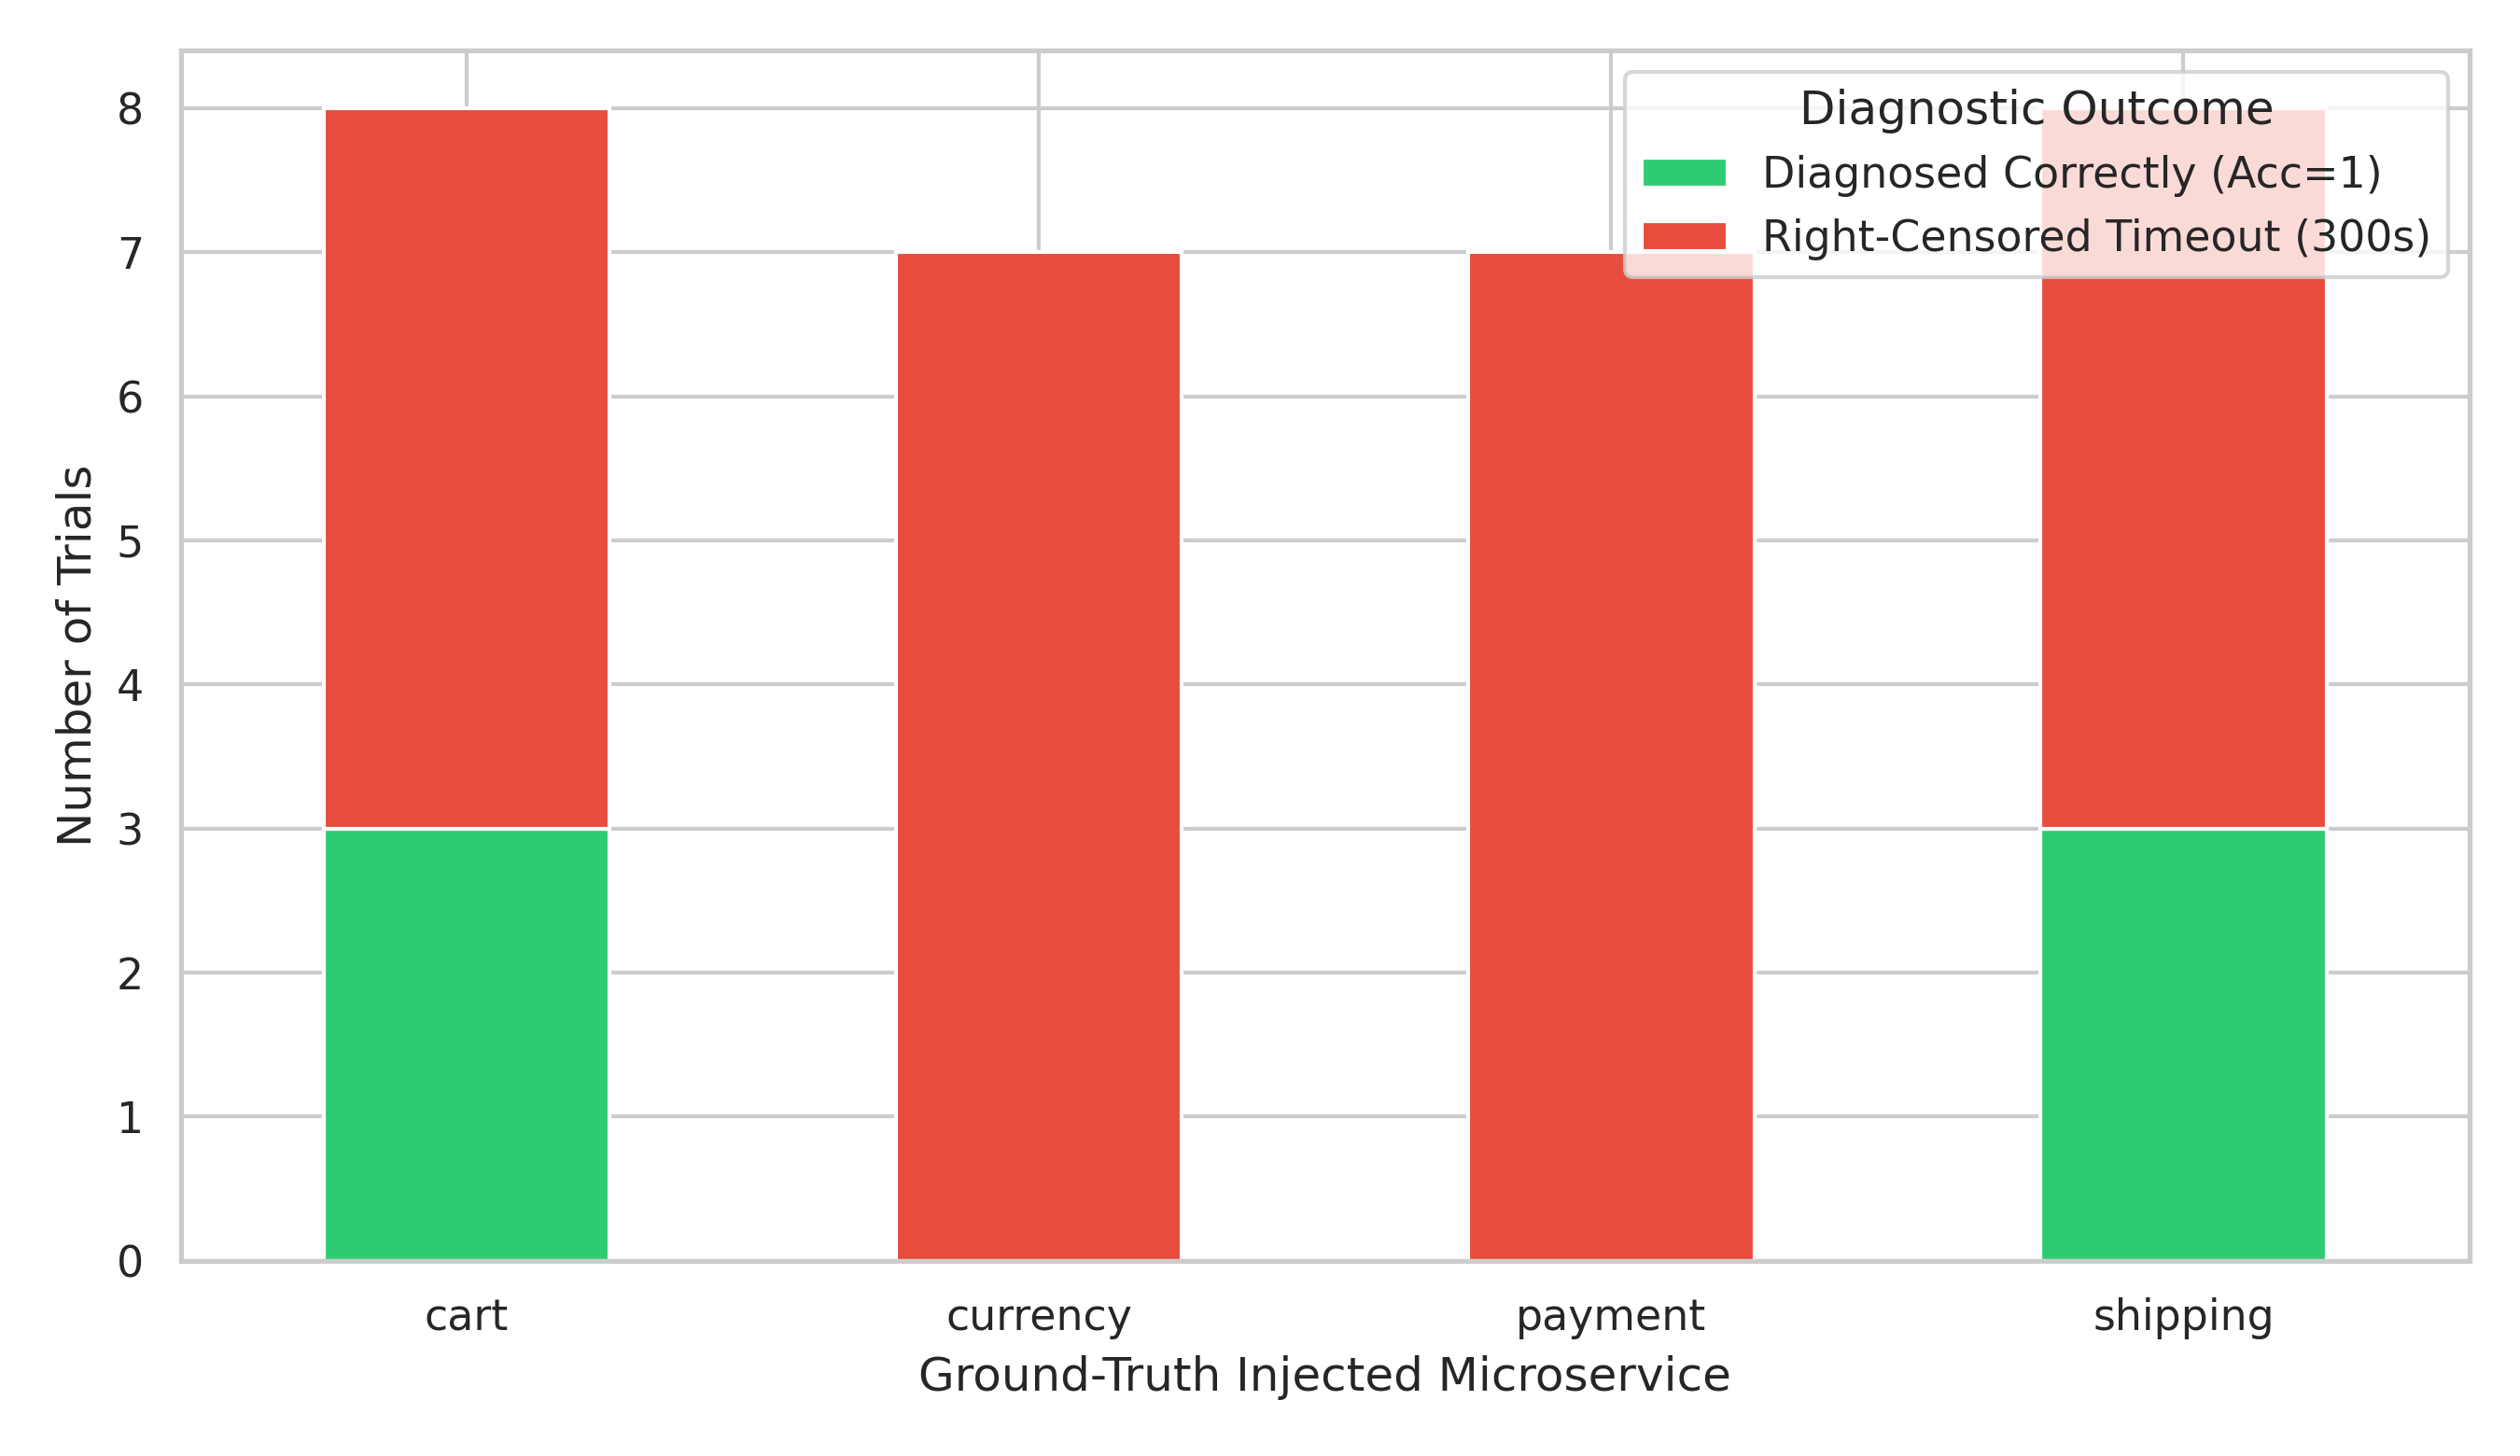
\includegraphics[height=0.35\textheight, keepaspectratio]{results/scenario3_outcomes.png}
    \end{column}
  \end{columns}
\end{frame}

\begin{frame}{O Estado Atual do Ecossistema Open-Source (CNCF)}
  \begin{columns}[T]
    \begin{column}{0.49\textwidth}
      \begin{block}{\textbf{Métricas: Prometheus}}
        \small
        \begin{itemize}
          \item Padrão de fato na CNCF para coleta de séries temporais numéricas via raspagem (\textit{pull});
          \item Mecanismo de consultas com PromQL para alertas e avaliação contínua de SLOs.
        \end{itemize}
      \end{block}
      \vspace{0.8ex}
      \begin{block}{\textbf{Logs: Grafana Loki}}
        \small
        \begin{itemize}
          \item Agregação horizontal e escalável de logs inspirada na arquitetura do Prometheus;
          \item Indexação minimalista exclusivamente por metadados de \textit{labels}, minimizando uso de RAM.
        \end{itemize}
      \end{block}
    \end{column}
    
    \begin{column}{0.49\textwidth}
      \begin{block}{\textbf{Traces: Grafana Tempo}}
        \small
        \begin{itemize}
          \item Armazenamento de rastreamento distribuído em larga escala;
          \item Arquitetura \textit{index-free} baseada em blocos de objetos, eliminando custos operacionais de índices.
        \end{itemize}
      \end{block}
      \vspace{0.8ex}
      \begin{block}{\textbf{Instrumentação: OpenTelemetry (OTel)}}
        \small
        \begin{itemize}
          \item Padrão unificado da indústria para APIs, SDKs e coletores de dados (\textit{vendor-neutral});
          \item Convenções semânticas padronizadas entre diferentes linguagens e plataformas.
        \end{itemize}
      \end{block}
    \end{column}
  \end{columns}
\end{frame}

\begin{frame}{Lacunas Arquiteturais \& A Missão do PANOPTES}
  \begin{columns}[T]
    \begin{column}{0.49\textwidth}
      \begin{alertblock}{\textbf{As 3 Grandes Lacunas Arquiteturais}}
        \small
        \begin{enumerate}
          \item \textbf{Fragmentação em Silos:} Cada ferramenta opera de forma isolada; ausência de uma arquitetura de referência formal e validada para Kubernetes;
          \vspace{0.5ex}
          \item \textbf{Integração Manual Complexa:} Dificuldade de propagação de contexto semântico unificado (\texttt{trace\_id}, tags de pods) entre métricas, logs e traces;
          \vspace{0.5ex}
          \item \textbf{O Efeito Observador:} Pilhas de monitoramento pesadas que competem por recursos e esgotam CPU e RAM nos nós de trabalho.
        \end{enumerate}
      \end{alertblock}
    \end{column}
    
    \begin{column}{0.49\textwidth}
      \begin{exampleblock}{\textbf{A Missão da Arquitetura PANOPTES}}
        \small
        \textbf{Unificação com Garantias Formais:}
        \begin{itemize}
          \item Harmonizar os componentes abertos da CNCF sob uma \textbf{arquitetura de referência reproduzível} (IaC com Helm e Ansible);
          \item Estabelecer \textbf{Princípios Formais de Controle} (\texttt{CP1}, \texttt{CP2}) para correlação semântica cruzada em tempo real;
          \item Aplicar \textbf{Heurísticas de Contingência} (\texttt{ConH1}--\texttt{ConH3}) para garantir envelope operacional de sobrecarga estritamente contido ($\Delta_{\text{CPU}} \le 15\%$, $\Delta_{\text{RAM}} \le 30\%$).
        \end{itemize}
      \end{exampleblock}
    \end{column}
  \end{columns}
\end{frame}

% ==============================================================================
% SECTION 2: RESEARCH QUESTIONS & OBJECTIVES
% ==============================================================================
\section{Perguntas de Pesquisa, Objetivos \& Hipóteses}

\begin{frame}{Perguntas de Pesquisa (RQs)}
  \begin{block}{\textbf{Questão Principal de Pesquisa (MRQ)}}
    \textit{Como uma arquitetura de referência para observabilidade em Kubernetes, fundamentada em padrões abertos, pode aprimorar a capacidade de diagnóstico de falhas em microsserviços em comparação aos mecanismos nativos de inspeção da plataforma?}
  \end{block}
  
  \vspace{1ex}
  \begin{columns}[T]
    \begin{column}{0.49\textwidth}
      \begin{exampleblock}{\textbf{SRQ1 (Requisitos Arquiteturais)}}
        \small Quais são os requisitos mínimos e componentes open-source para uma camada completa ($\mathcal{O} = \{M, L, T, E\}$) em orquestradores Kubernetes?
      \end{exampleblock}
      \vspace{0.5ex}
      \begin{exampleblock}{\textbf{SRQ2 (Integração \& Overhead)}}
        \small Como instanciar uma arquitetura com ferramentas abertas garantindo integração semântica sem sobrecarregar os recursos do cluster?
      \end{exampleblock}
    \end{column}
    
    \begin{column}{0.49\textwidth}
      \begin{exampleblock}{\textbf{SRQ3 (Eficácia Diagnóstica \& RCA)}}
        \small Qual o impacto na detecção e diagnóstico de causa-raiz ($MTTDiag$ e $Acc$) sob falhas induzidas em relação ao Kubernetes Vanilla?
      \end{exampleblock}
      \vspace{0.5ex}
      \begin{exampleblock}{\textbf{SRQ4 (Maturidade \& Classificação)}}
        \small Como classificar os estágios evolutivos de observabilidade e quais as lacunas presentes nas implementações atuais?
      \end{exampleblock}
    \end{column}
  \end{columns}
\end{frame}

\begin{frame}{Objetivos da Pesquisa (Geral e Específicos)}
  \begin{block}{Objetivo Geral}
    \textbf{Propor, instanciar e validar empiricamente} uma arquitetura de referência de observabilidade (\textbf{PANOPTES}) baseada em padrões abertos da CNCF para microsserviços em ecossistemas Kubernetes.
  \end{block}
  
  \vspace{0.8ex}
  \begin{columns}[T]
    \begin{column}{0.49\textwidth}
      \begin{exampleblock}{\textbf{SO1 (Estado da Arte \& Requisitos)}}
        \small Mapear a literatura e sintetizar requisitos arquiteturais de observabilidade para Kubernetes via Rapid Review.
      \end{exampleblock}
      \vspace{0.5ex}
      \begin{exampleblock}{\textbf{SO2 (Concepção Arquitetural)}}
        \small Conceber a arquitetura de referência PANOPTES fundamentada em princípios de controle (CP1, CP2) e padrões OTel.
      \end{exampleblock}
    \end{column}
    
    \begin{column}{0.49\textwidth}
      \begin{exampleblock}{\textbf{SO3 (Instanciação em Testbed)}}
        \small Implementar a pilha como IaC (Ansible/Helm) em ambiente controlado multi-nó com microsserviços benchmark.
      \end{exampleblock}
      \vspace{0.5ex}
      \begin{exampleblock}{\textbf{SO4 (Validação Experimental)}}
        \small Avaliar empiricamente eficácia diagnóstica ($MTTDiag$, $Acc$) e limites de sobrecarga sob Chaos Engineering.
      \end{exampleblock}
    \end{column}
  \end{columns}
\end{frame}

\begin{frame}{Hipóteses Formais de Pesquisa}
  \small
  As hipóteses avaliam o ganho de eficácia diagnóstica e a contenção do \textit{Efeito Observador}:
  \vspace{0.8ex}

  \begin{columns}[T]
    \begin{column}{0.32\textwidth}
      \begin{alertblock}{Hipótese $H_{1,1}$ ($MTTDiag$)}
        \footnotesize
        \textbf{Latência de Diagnóstico:}\\
        A correlação multimodal reduz significativamente o tempo médio de diagnóstico sob falhas latentes:
        \vspace{-1ex}
        \begin{equation*}
          \mu(MTTDiag_{\text{P}}) < \mu(MTTDiag_{\text{V}})
        \end{equation*}
        \vspace{-1.5ex}
        \begin{itemize}
          \item Teste: Wilcoxon/Mann-Whitney;
          \item Significância: $\alpha = 0.05$.
        \end{itemize}
      \end{alertblock}
    \end{column}
    
    \begin{column}{0.32\textwidth}
      \begin{alertblock}{Hipótese $H_{1,2}$ ($Acc$)}
        \footnotesize
        \textbf{Acurácia Diagnóstica:}\\
        A identificação da causa-raiz é estatisticamente superior à inspeção Vanilla CLI:
        \vspace{-1ex}
        \begin{equation*}
          Acc_{\text{PANOPTES}} > Acc_{\text{Vanilla}}
        \end{equation*}
        \vspace{-1.5ex}
        \begin{itemize}
          \item Teste exato de Fisher;
          \item Cenários de falhas latentes.
        \end{itemize}
      \end{alertblock}
    \end{column}
    
    \begin{column}{0.32\textwidth}
      \begin{alertblock}{Hipótese $H_{1,3}$ (Overhead)}
        \footnotesize
        \textbf{Sobrecarga Delimitada:}\\
        A sobrecarga do sistema de telemetria mantém-se contida no envelope seguro:
        \vspace{-1ex}
        \begin{align*}
          \Delta_{\text{CPU}} &\le 15\% \ (\text{workload})\\
          \Delta_{\text{RAM}} &\le 30\% \ (\text{cluster})
        \end{align*}
        \vspace{-1.5ex}
        \begin{itemize}
          \item Bounded Observer Effect;
          \item Proteção dos nós de trabalho.
        \end{itemize}
      \end{alertblock}
    \end{column}
  \end{columns}
\end{frame}

% ==============================================================================
% SECTION 3: METHODOLOGICAL FRAMEWORK & STATE OF THE ART
% ==============================================================================
\section{Metodologia \& Estado da Arte}

\begin{frame}{Metodologia: Ciclo de Vida DSRM (Peffers et al., 2006)}
  \begin{columns}[T]
    \begin{column}{0.48\textwidth}
      \begin{block}{1. Identificação do Problema}
        \small Fragilidade do diagnóstico operacional e fragmentação telemétrica (métricas, logs e traces) em Kubernetes.
      \end{block}
      \vspace{0.6ex}
      \begin{block}{2. Definição dos Objetivos}
        \small Requisitos formais para observabilidade aberta unificada e correlação multimodal sem silos proprietários.
      \end{block}
      \vspace{0.6ex}
      \begin{block}{3. Design \& Desenvolvimento}
        \small Arquitetura PANOPTES, correlacionador multimodal e automação IaC reprodutível (Ansible/Helm).
      \end{block}
    \end{column}
    
    \begin{column}{0.48\textwidth}
      \begin{block}{4. Demonstração}
        \small Testbed emulador K3d multi-nó instrumentado com isolamento estrito de contêineres via cgroups.
      \end{block}
      \vspace{0.6ex}
      \begin{block}{5. Avaliação Experimental}
        \small Injeção sistemática de falhas (Chaos Mesh) sob design fatorial $2\times2$ com cargas sintéticas.
      \end{block}
      \vspace{0.6ex}
      \begin{block}{6. Comunicação \& Transferência}
        \small Decisões arquiteturais registradas (MADRs), artigos científicos e repositório open-source.
      \end{block}
    \end{column}
  \end{columns}
\end{frame}

\begin{frame}{Metodologia: Os Três Ciclos de Pesquisa DSR (Hevner et al., 2004)}
  \begin{columns}[T]
    \begin{column}{0.48\textwidth}
      \begin{exampleblock}{Ciclos de Pesquisa (Hevner et al., 2004)}
        \small
        Articulação rigorosa entre relevância prática, rigor científico e projeto do artefato:
        \begin{itemize}
          \item \textbf{Ciclo de Relevância (\textit{Relevance}):}\\
          Conecta o ambiente do problema (orquestração Kubernetes, complexidade operacional e requisitos CNCF) aos requisitos e critérios de aceitação.
          \item \textbf{Ciclo de Rigor (\textit{Rigor}):}\\
          Garante fundamentação na Teoria de Controle (Kalman), Engenharia de Caos e na literatura formal de observabilidade.
          \item \textbf{Ciclo de Design (\textit{Design}):}\\
          Núcleo iterativo de construção do artefato PANOPTES e validação experimental controlada.
        \end{itemize}
      \end{exampleblock}
    \end{column}
    
    \begin{column}{0.48\textwidth}
      \centering
      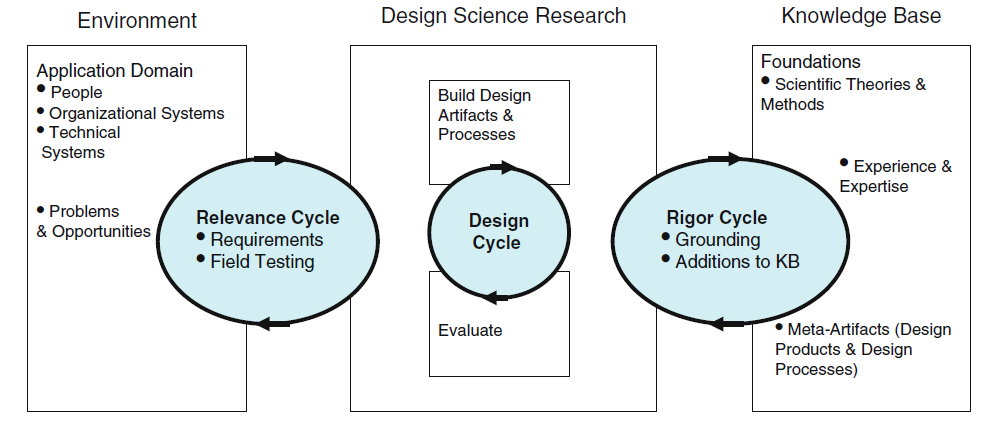
\includegraphics[width=\linewidth, keepaspectratio]{methodology/hevner-dsr-cycles.png}
      \vspace{0.6ex}
      \begin{block}{Interação entre os Ciclos}
        \footnotesize
        \begin{itemize}
          \item \textbf{Retroalimentação Contínua:} Evidências experimentais refinam tanto a teoria formal quanto o contexto operacional;
          \item \textbf{Artefato Prescritivo:} PANOPTES materializa princípios de controle testáveis e replicáveis.
        \end{itemize}
      \end{block}
    \end{column}
  \end{columns}
\end{frame}

\begin{frame}{Estado da Arte: Protocolo da Rapid Review Sistemática}
  \begin{columns}[T]
    \begin{column}{0.49\textwidth}
      \begin{block}{Protocolo de Pesquisa \& Diretrizes}
        \small
        \begin{itemize}
          \item \textbf{Diretrizes:} Cartaxo et al. (2018) e Kitchenham; síntese ágil e rigorosa de evidências sem a latência de uma RSL.
          \item \textbf{Gestão Metodológica:} Plataforma \textit{Parsifal} para auditoria, extração e reprodutibilidade.
          \item \textbf{Bases Indexadas ($N = 312$, 2018--2025):}\\
          IEEE Xplore ($114$), ACM DL ($88$), SpringerLink ($68$) e ScienceDirect ($42$).
          \item \textbf{String Canônica:} \textit{(cloud-native OR microservices) AND (observability OR metrics OR logs OR traces) AND (kubernetes) AND (open-source)}.
        \end{itemize}
      \end{block}
    \end{column}
    
    \begin{column}{0.47\textwidth}
      \begin{block}{Funil PRISMA ($N = 10$ Primários)}
        \small
        \begin{itemize}
          \item \textbf{Identificação:} $312$ registros nas bases;
          \item \textbf{Deduplicação:} $58$ removidos ($254$ únicos);
          \item \textbf{Elegibilidade:} $46$ estudos em texto completo;
          \item \textbf{Síntese Final:} \textbf{10 estudos} (8 diretos $+ 2$ via snowballing com $\text{QA} \ge 3.5$).
        \end{itemize}
      \end{block}
      \vspace{0.4ex}
      \begin{exampleblock}{Questões de Revisão Investigadas}
        \scriptsize
        \textbf{RQ01:} Componentes essenciais ($O = \{M, L, T, E\}$);\\[1pt]
        \textbf{RQ02:} Arquiteturas de referência para Kubernetes;\\[1pt]
        \textbf{RQ03:} Ferramentas open-source (OTel, Loki, Tempo);\\[1pt]
        \textbf{RQ04:} Lacunas arquiteturais e direções futuras.
      \end{exampleblock}
    \end{column}
  \end{columns}
\end{frame}

\begin{frame}{Estado da Arte: Lacunas da Literatura \& Contribuições}
  \begin{columns}[T]
    \begin{column}{0.48\textwidth}
      \begin{alertblock}{Identificação da "Lacuna de Validação"}
        \small
        \textbf{Diagnóstico da Literatura (Wendler, 2012):}
        \begin{itemize}
          \item \textbf{Predomínio Conceitual:} Alta concentração de propostas teóricas sem medição rigorosa de desempenho;
          \item \textbf{Escassez de Benchmarks:} Falta de testbeds reproduzíveis com injeção sistemática de falhas em cascata;
          \item \textbf{Vazio Normativo:} Inexistência de modelos estruturados para guiar e mensurar a maturidade de observabilidade.
        \end{itemize}
      \end{alertblock}
    \end{column}
    
    \begin{column}{0.48\textwidth}
      \begin{exampleblock}{Contribuição Direta Desta Tese}
        \small
        \textbf{Resposta Concreta às Lacunas da Literatura:}
        \begin{itemize}
          \item \textbf{Modelo de Maturidade (OMM):} 5 níveis formais baseados em Becker et al. (2009) para avaliar e evoluir clusters K8s;
          \item \textbf{Arquitetura PANOPTES:} Referência aberta instanciando o \textbf{Nível 4 (Optimized)} com pipelines OTLP;
          \item \textbf{Validação com Chaos Engineering:} Avaliação empírica via design fatorial $2\times2$ sob falhas latentes induzidas.
        \end{itemize}
      \end{exampleblock}
    \end{column}
  \end{columns}
\end{frame}

\begin{frame}{O Modelo de Maturidade de Observabilidade (OMM)}
  \begin{block}{Formalização de 5 Níveis Evolutivos (Grounded em Becker et al., 2009)}
    Estruturado para guiar a adoção prática e preencher a lacuna teórica na literatura:
  \end{block}
  
  \small
  \begin{tabularx}{\textwidth}{c p{2.8cm} X p{3.2cm}}
    \toprule
    \textbf{Nível} & \textbf{Estágio} & \textbf{Características Operacionais} & \textbf{Diagnóstico / RCA} \\
    \midrule
    \textbf{L1} & \textbf{Non-Existent} & Ausência de instrumentação. Falhas detectadas por usuários finais. & Puramente reativo. \\
    \addlinespace
    \textbf{L2} & \textbf{Initial / Ad-Hoc} & Comandos CLI pontuais (\texttt{kubectl logs/top}). Telemetria efêmera sem persistência. & Manual, lento, $20\%$ acurácia. \\
    \addlinespace
    \textbf{L3} & \textbf{Managed Silos} & Coletores isolados (Prometheus OU Jaeger). Ausência de vínculos semânticos cruzados. & Falha sob traces em cascata ($0\%$ acc). \\
    \addlinespace
    \rowcolor{cinRed!12}
    \textbf{L4} & \textbf{\textbf{Optimized (PANOPTES)}} & \textbf{Correlação multimodal (M, L, T). Decomposição de self-time e OTLP resource attributes.} & \textbf{Automatizado, $83.3\%$ acc, $MTTDiag = 17\,\text{s}$.} \\
    \addlinespace
    \textbf{L5} & \textbf{Predictive / Autonomic} & AIOps, modelos preditivos em tempo real e self-healing acoplado ao plano de controle K8s. & Fechamento de ciclo de controle autônomo. \\
    \bottomrule
  \end{tabularx}
\end{frame}

% ==============================================================================
% SECTION 4: THE PANOPTES ARCHITECTURE & ADRS
% ==============================================================================
\section{A Arquitetura de Referência PANOPTES}

\begin{frame}{Visão Geral da Arquitetura PANOPTES}
  \vspace{-1ex}
  \begin{columns}[T]
    \begin{column}{0.24\textwidth}
      \begin{block}{\scriptsize 1. Coleta no Host/Nó}
        \tiny
        \textbf{OTel Collector DaemonSet}\\
        Captura métricas cgroups, kubelet e logs de pods via OTLP em nível de nó.
      \end{block}
    \end{column}
    \begin{column}{0.24\textwidth}
      \begin{block}{\scriptsize 2. Normalização}
        \tiny
        \textbf{Processadores \& Tags}\\
        Enriquecimento semântico padronizado (\texttt{service.name}, \texttt{k8s.pod.name}, \texttt{trace\_id}).
      \end{block}
    \end{column}
    \begin{column}{0.26\textwidth}
      \begin{block}{\scriptsize 3. Backends Dedicados}
        \tiny
        \textbf{Armazenamento Especializado:}\\
        $\bullet$ \textbf{Prometheus:} Séries (pull)\\
        $\bullet$ \textbf{Loki:} Logs index-by-label\\
        $\bullet$ \textbf{Tempo:} Traces (index-free)
      \end{block}
    \end{column}
    \begin{column}{0.24\textwidth}
      \begin{block}{\scriptsize 4. Correlação \& RCA}
        \tiny
        \textbf{Painéis \& APIs Unificadas}\\
        Visualização integrada (Grafana) e consultas correlacionadas (PromQL, LogQL, TraceQL).
      \end{block}
    \end{column}
  \end{columns}
  
  \vspace{0.8ex}
  \centering
  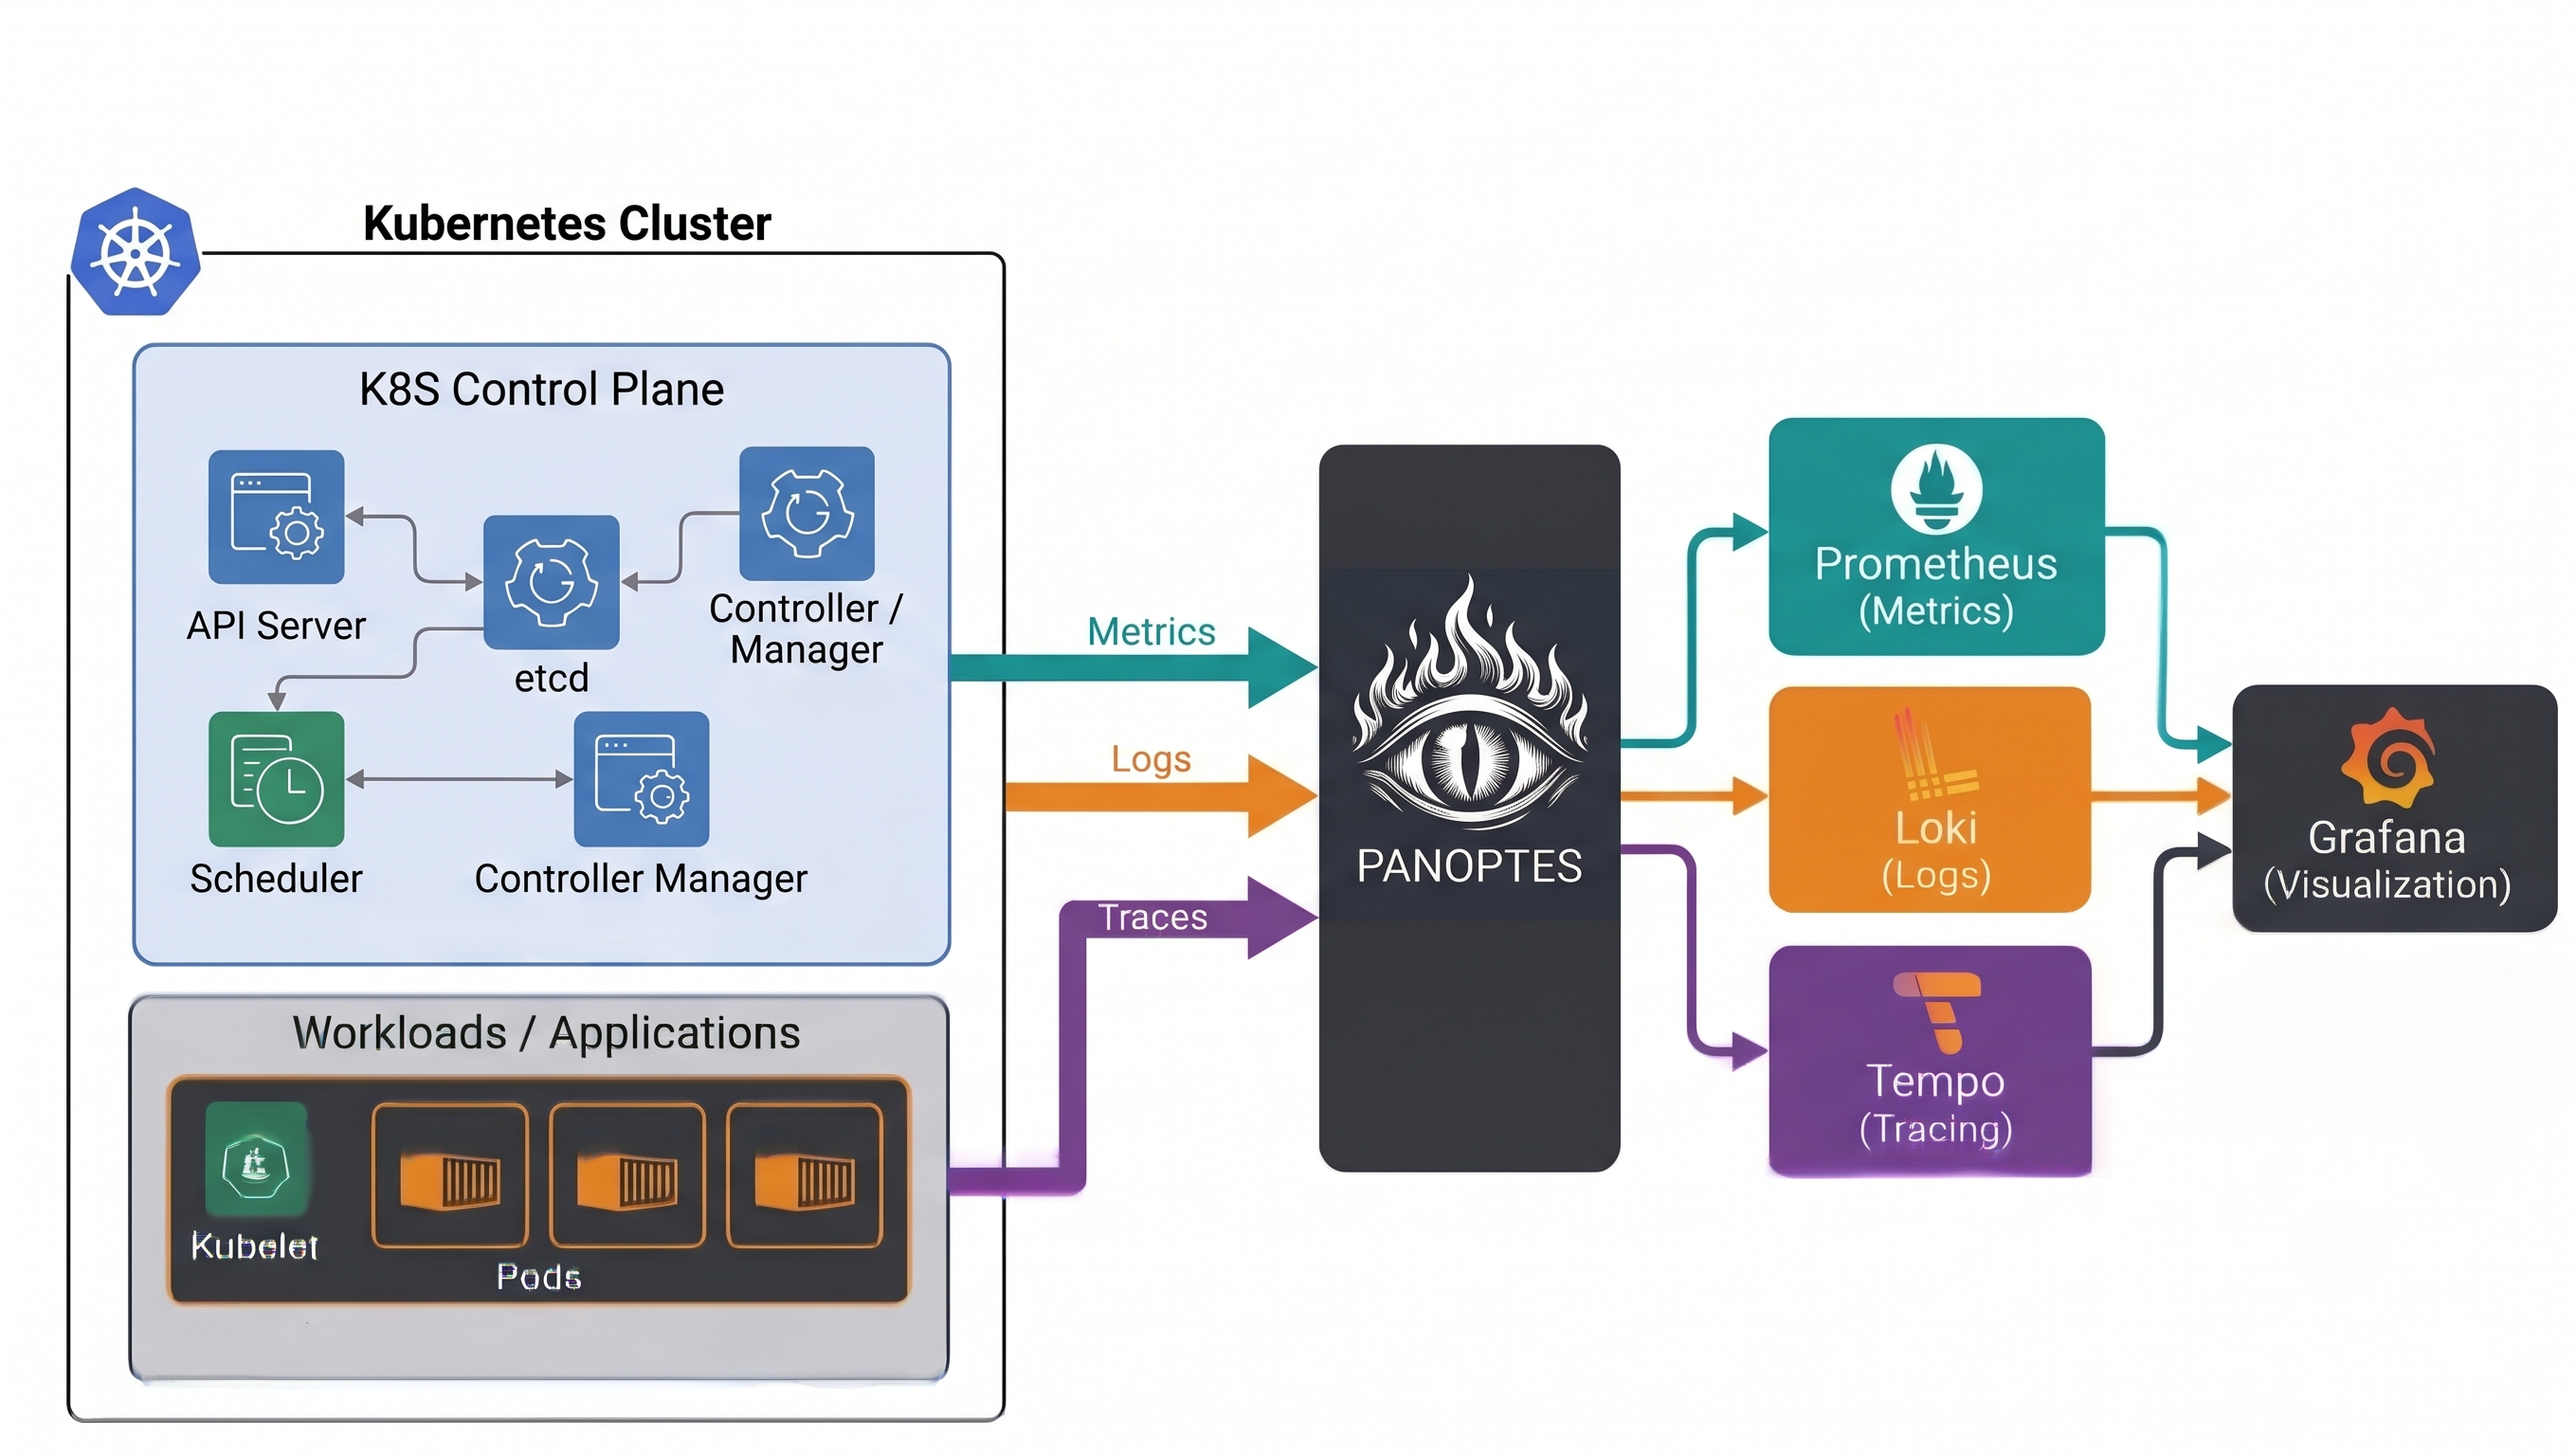
\includegraphics[height=0.48\textheight, keepaspectratio]{experiment/panoptes_architecture.png}
\end{frame}

\begin{frame}{Princípios de Controle (CPs) \& Heurísticas de Contingência (ConHs)}
  \begin{columns}[T]
    \begin{column}{0.5\textwidth}
      \begin{exampleblock}{Princípios de Controle (Fundamentação Teórica)}
        \begin{itemize}
          \item \textbf{CP1 (Vínculo Causal):} Vínculo contextual explícito entre métricas, logs e traces via identificadores W3C (\texttt{trace\_id}) e \textit{exemplars} em histogramas.
          \item \textbf{CP2 (Representação Unificada do Estado):} Identidade dimensional canônica compartilhada entre sinais através de convenções OTLP e metadados de orquestração do Kubernetes.
        \end{itemize}
      \end{exampleblock}
    \end{column}
    
    \begin{column}{0.5\textwidth}
      \begin{alertblock}{Heurísticas de Contingência (Engenharia \& Sobrecarga)}
        \begin{itemize}
          \item \textbf{ConH1 (Controle Declarativo):} Toda a topologia gerenciada via Infrastructure as Code (IaC) e GitOps determinístico.
          \item \textbf{ConH2 (Rejeição de Desvio):} Tratamento do desvio de configuração (\textit{drift}) como perturbação a ser anulada.
          \item \textbf{ConH3 (Feedback Adaptativo / Bounded Overhead):} Proteção contra o \textit{Efeito Observador} via batching OTel e armazenamento index-free.
        \end{itemize}
      \end{alertblock}
    \end{column}
  \end{columns}
\end{frame}

\begin{frame}{Decisões Arquiteturais Registradas (MADR-0001 a MADR-0006)}
  \small
  \begin{tabularx}{\textwidth}{l p{3.2cm} X l}
    \toprule
    \textbf{ADR} & \textbf{Decisão} & \textbf{Racional Metodológico \& Impacto} & \textbf{Validade} \\
    \midrule
    \textbf{0001} & Design Pareado Estratificado & Agendamento balanceado (\texttt{SEED=42}; 10 de cada tipo de falha) e cadência de polling idêntica ($4\,\text{s}$). Permite Wilcoxon e McNemar pareados. & Conclusão \\
    \addlinespace
    \textbf{0002} & Eliminação de Data Leakage & Removido fallback a CLI. Operação exclusiva via APIs HTTP de telemetria e \textit{decomposição de self-time} de traces. & Construto \\
    \addlinespace
    \textbf{0003} & Intervalo Anti-Pseudoreplicação & Aumento do profiling para $16\,\text{s}$ (excedendo a janela de $15\,\text{s}$ do \texttt{metrics-server}), eliminando autocorrelação artificial. & Estatística \\
    \addlinespace
    \textbf{0004} & Isolamento Chaos Mesh & Injeção direcionada (\texttt{direction: to}) e binding específico a pods (\texttt{cart} vs \texttt{valkey-cart}), com sanitização de finalizers. & Interna \\
    \addlinespace
    \textbf{0005} & Poda de Workload Não-Essencial & Desativação de 8 pods de background da demo OTel, recuperando $1.86\,\text{GiB}$ RAM e evitando thrashing de memória virtual (\texttt{kswapd0}). & Interna \\
    \addlinespace
    \textbf{0006} & Evolução de Virtualização & Migração de Vagrant/VirtualBox e Multipass para \textbf{K3d nativo no WSL2} com cotas rígidas de \texttt{cgroups} ($2.0\text{ CPU}, 4\text{G RAM}$/nó). & Conclusão \\
    \bottomrule
  \end{tabularx}
\end{frame}

% ==============================================================================
% SECTION 5: EXPERIMENTAL DESIGN & CHAOS CAMPAIGNS
% ==============================================================================
\section{Design Experimental \& Campanhas de Chaos Engineering}

\begin{frame}{Design Fatorial $2 \times 2$ \& Ambiente Experimental}
  \begin{columns}[T]
    \begin{column}{0.5\textwidth}
      \begin{block}{Matriz Fatorial $2 \times 2$}
        \centering
        \resizebox{\linewidth}{!}{%
        \begin{tabular}{c|c|c}
          & \textbf{Vanilla K8s} & \textbf{PANOPTES} \\ \hline
          \textbf{Steady-State} & \textbf{Cenário 1} & \textbf{Cenário 2} \\
          (Carga Contínua) & (Baseline Overhead) & (Overhead PANOPTES) \\ \hline
          \textbf{Chaos Injection} & \textbf{Cenário 3 / 3-Strat} & \textbf{Cenário 4b} \\
          (Falhas Latentes) & (CLI Baseline) & (Multimodal RCA)
        \end{tabular}%
        }
      \end{block}
      \vspace{-0.5ex}
      \begin{exampleblock}{Cenário Adicional Exploratório}
        \small \textbf{Cenário 4a:} Rastreamento distribuído monomodal isolado (sem correlação multimodal).
      \end{exampleblock}
    \end{column}
    
    \begin{column}{0.48\textwidth}
      \begin{alertblock}{Infraestrutura do Testbed (K3d)}
        \small
        \begin{itemize}
          \item \textbf{Cluster Multi-Node:} 1 Server + 2 Agents;
          \item \textbf{Isolamento por cgroups:} Limites de $2.0\,\text{vCPU}$ e $4.0\,\text{GiB}$ RAM/nó;
          \item \textbf{Carga Alvo:} CNCF Astronomy Shop (\texttt{otel-demo});
          \item \textbf{Gerador de Carga:} Locust em loop contínuo de e-commerce.
        \end{itemize}
      \end{alertblock}
    \end{column}
  \end{columns}
\end{frame}

\begin{frame}{Protocolo de Injeção de Falhas (Chaos Mesh)}
  \begin{columns}[T]
    \begin{column}{0.58\textwidth}
      \begin{block}{Taxonomia das Perturbações Injetadas ($N=30$ ensaios)}
        \begin{enumerate}
          \item \textbf{\texttt{cpu-stress} ($n=10$):} Consumo forçado de $100\%$ da cota de CPU no pod alvo (induz contenção e throttling de ciclos).
          \item \textbf{\texttt{network-delay} ($n=10$):} Injeção de $1500\,\text{ms}$ de latência com jitter de $100\,\text{ms}$ no tráfego de saída do microsserviço.
          \item \textbf{\texttt{pod-kill} ($n=10$):} Envio de sinal \texttt{SIGKILL} abrupto, simulando falha de hardware ou terminação brusca por OOMKilled.
        \end{enumerate}
      \end{block}
      
      \begin{exampleblock}{Rigor Metodológico}
        \begin{itemize}
          \item Semente pseudoaleatória reproduzível (\texttt{RANDOM\_SEED = 42});
          \item Timeout de censura à direita fixado em $300\,\text{s}$;
          \item Tempo de estabilização pós-falha (\textit{cooldown}) entre rodadas.
        \end{itemize}
      \end{exampleblock}
    \end{column}
    
    \begin{column}{0.4\textwidth}
      \begin{alertblock}{Métricas Primárias}
        \begin{itemize}
          \item \textbf{$MTTDiag$ (s):}\\
            Tempo transcorrido desde $T_0$ (injeção) até o registro objetivo da causa-raiz.
          \item \textbf{$Acc$ (\%):}\\
            Taxa de acertos exatos do pod e falha injetada ($TP / N$).
          \item \textbf{Censura (\%):}\\
            Ensaios que atingiram $300\,\text{s}$ sem resolução.
        \end{itemize}
      \end{alertblock}
    \end{column}
  \end{columns}
\end{frame}

\begin{frame}{O Viés de Duração em Cascata: Por que o Tracing Isolado Falhou?}
  \begin{columns}[T]
    \begin{column}{0.52\textwidth}
      \begin{alertblock}{A Falha Crítica do Cenário 4a ($Acc = 0.00\%$)}
        \begin{itemize}
          \item No rastreamento monomodal convencional, a árvore de spans propaga a duração cumulativa de forma síncrona.
          \item \textbf{O Efeito Cascata:} O span do \texttt{frontend} ou \texttt{ingress} inclui a duração de todas as chamadas filhas!
          \item \textbf{Consequência:} Um algoritmo que busca apenas o span com maior duração ($T_{\text{span}}$) sempre aponta o gateway como culpado ($30/30$ atribuições errôneas!).
        \end{itemize}
      \end{alertblock}
    \end{column}
    
    \begin{column}{0.46\textwidth}
      \begin{exampleblock}{A Solução PANOPTES (Decomposição de Self-Time)}
        O motor PANOPTES calcula o \textbf{Tempo Exclusivo (\textit{Self-Time})}:
        \begin{equation*}
          T_{\text{self}} = T_{\text{span}} - \sum_{c \in \text{children}} T_c
        \end{equation*}
        \begin{itemize}
          \item Isola o tempo gasto estritamente no código do nó atual;
          \item Vincula atributos de cliente L4/L7 (\texttt{net.peer.name});
          \item Cruza com saturação de CPU (PromQL) e término de processo (LogQL).
        \end{itemize}
      \end{exampleblock}
    \end{column}
  \end{columns}
\end{frame}

% ==============================================================================
% SECTION 6: EMPIRICAL RESULTS & HYPOTHESIS TESTING
% ==============================================================================
\section{Resultados Empíricos \& Validação de Hipóteses}

\begin{frame}{Hipótese $H_{1,3}$: Sobrecarga de CPU no Workload}
  \begin{columns}[T]
    \begin{column}{0.48\textwidth}
      \begin{block}{Envelope de CPU ($\Delta_{\text{CPU}} \le 15\%$)}
        \footnotesize
        \begin{itemize}
          \item \textbf{Métrica:} Consumo relativo da pilha PANOPTES sobre o workload ativo ($1{,}994\,\text{mCPU}$).
          \item \textbf{Consumo Médio:} $189.5\,\text{mCPU}$ ($\mathbf{9.51\% \pm 2.14\%}$).
          \item \textbf{Mediana:} $\mathbf{8.83\%}$, estritamente abaixo do teto operacional de $15\%$.
        \end{itemize}
      \end{block}
      \vspace{0.3ex}
      \begin{alertblock}{Validação Estatística (Wilcoxon)}
        \footnotesize
        \begin{itemize}
          \item \textbf{Teste Monocaudal:} $H_{0}: \mu(\Delta_{\text{CPU}}) \ge 15\%$
          \item \textbf{Estatística:} $W = 0.0$
          \item \textbf{P-valor:} $\mathbf{p = 6.52 \times 10^{-9}}$
          \item \textbf{Conclusão:} Rejeição categórica de $H_{0}$; sobrecarga de CPU contida!
        \end{itemize}
      \end{alertblock}
    \end{column}
    
    \begin{column}{0.50\textwidth}
      \centering
      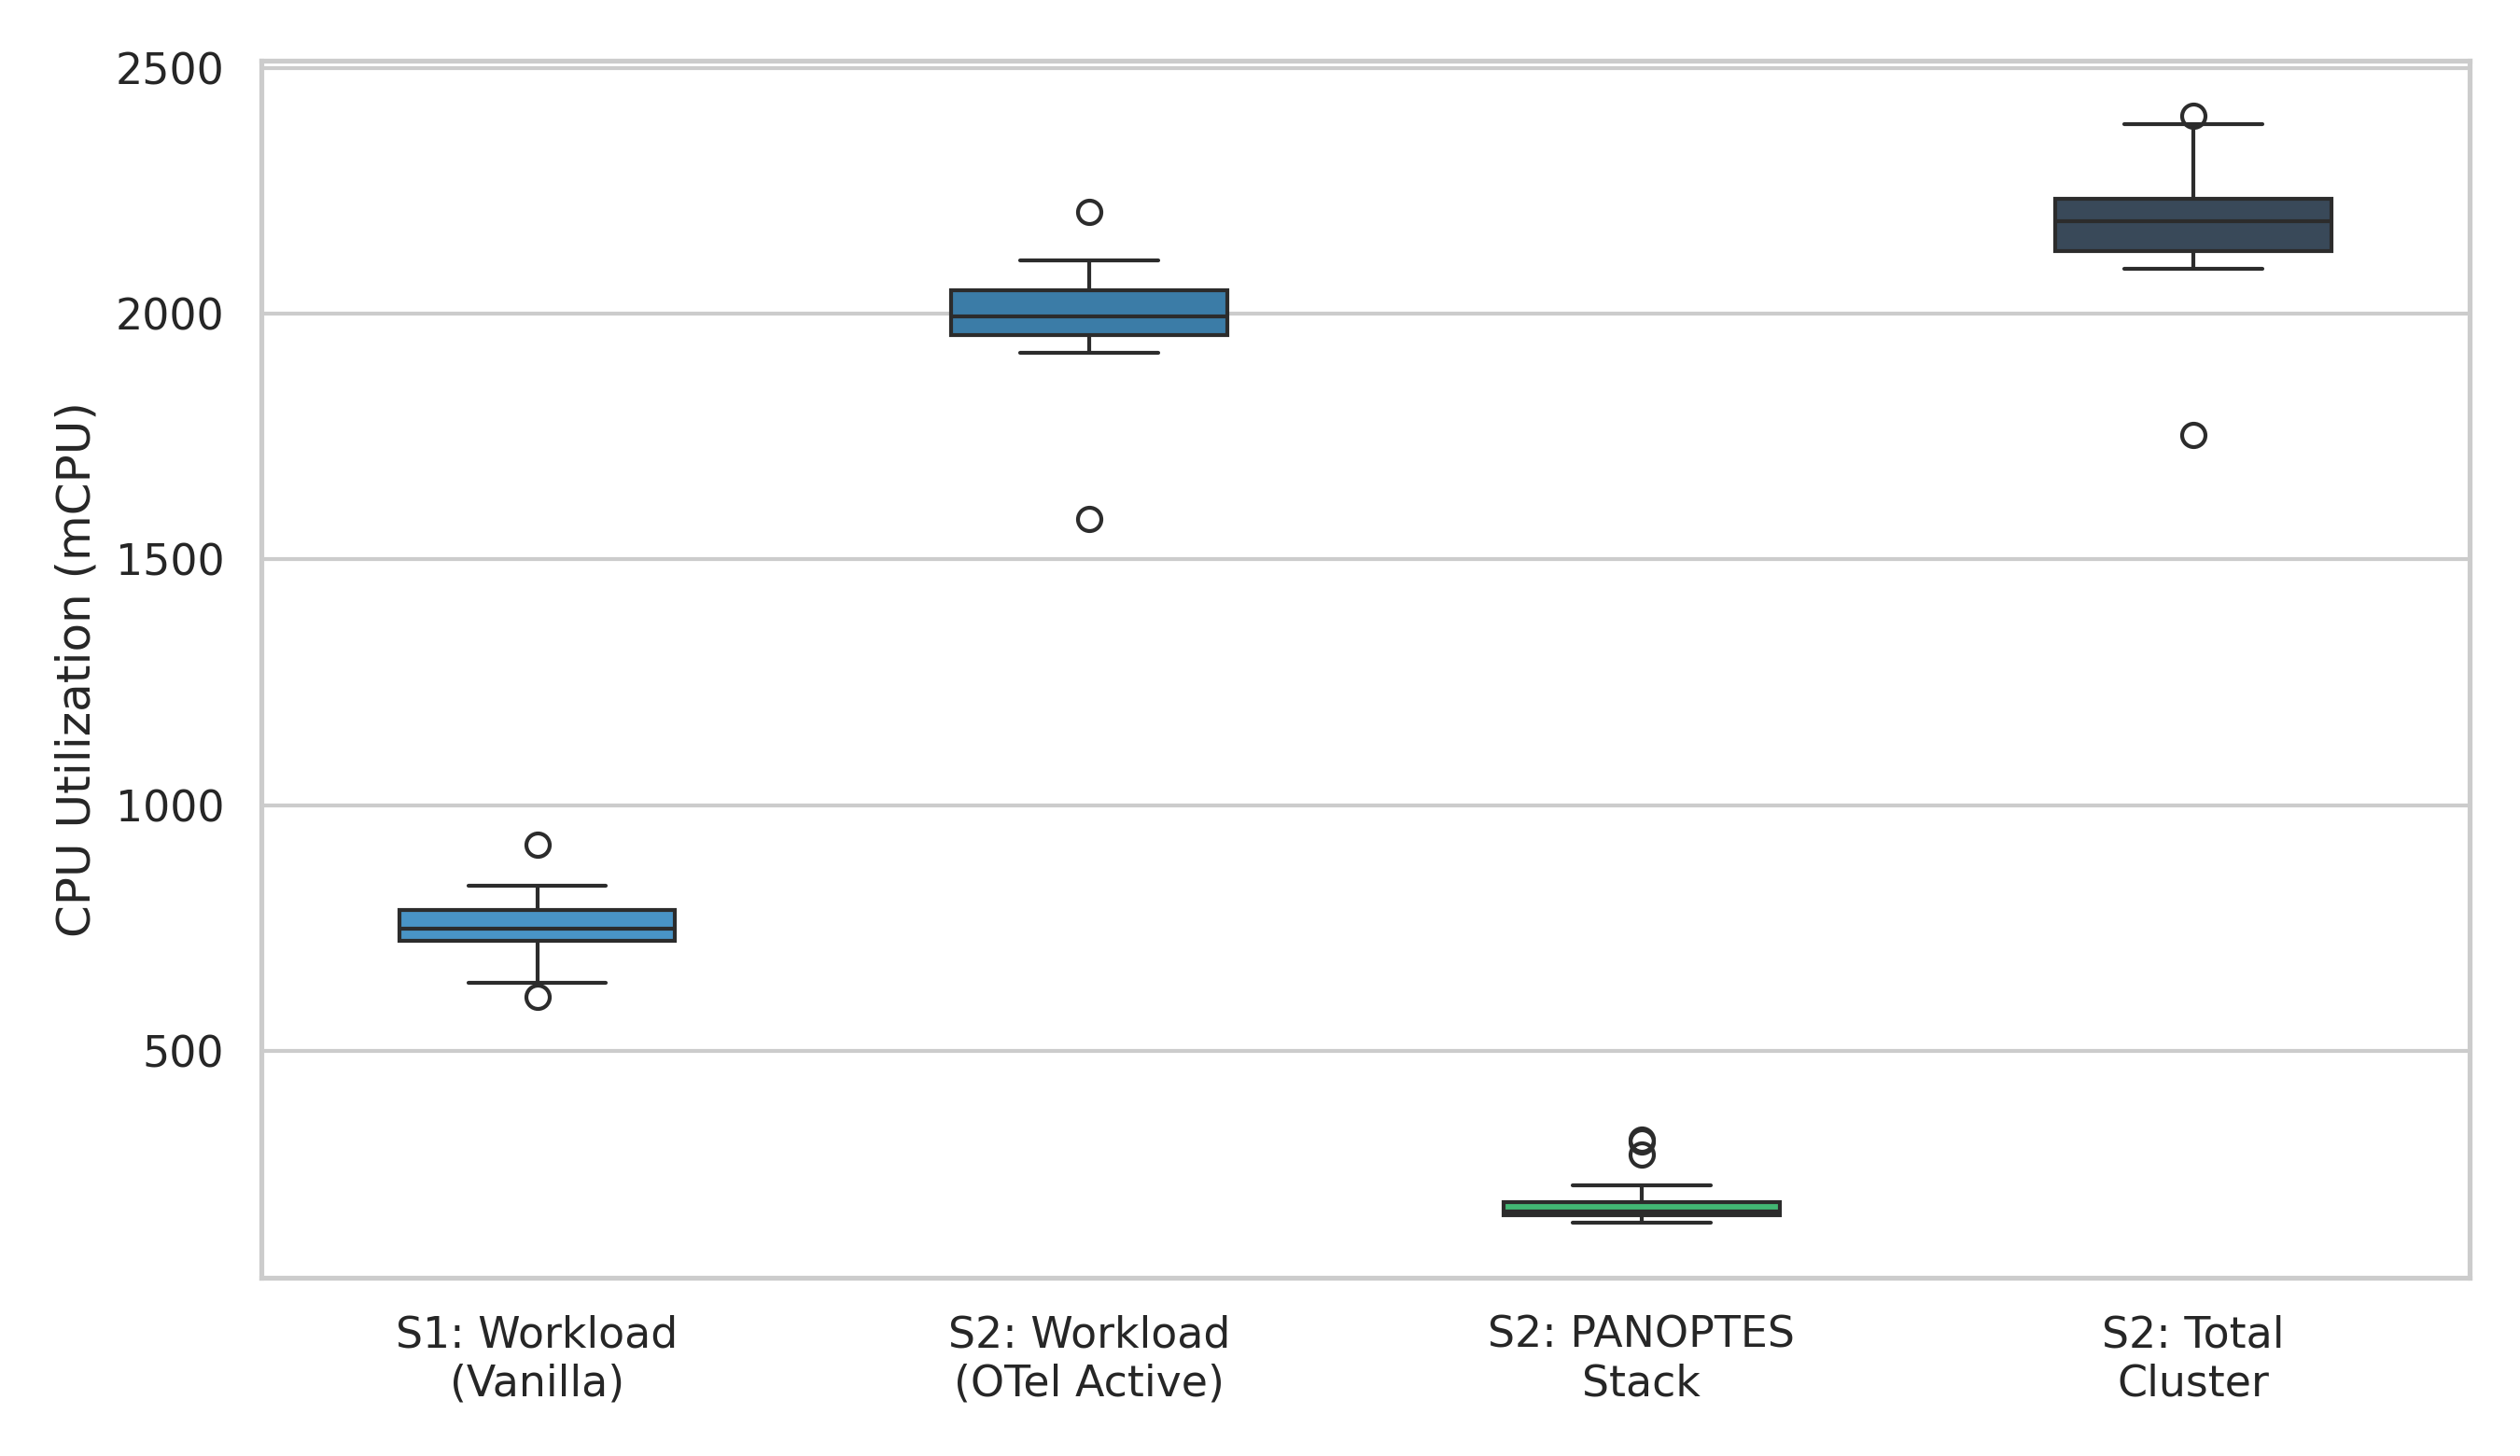
\includegraphics[width=\linewidth, keepaspectratio]{results/scenario2_cpu_overhead.png}
    \end{column}
  \end{columns}
\end{frame}

\begin{frame}{Hipótese $H_{1,3}$: Pegada de Memória RAM no Cluster}
  \begin{columns}[T]
    \begin{column}{0.48\textwidth}
      \begin{block}{Envelope de RAM ($\Delta_{\text{RAM}} \le 30\%$)}
        \footnotesize
        \begin{itemize}
          \item \textbf{Métrica:} Memória residente (RSS) de toda a pilha sobre a capacidade total do cluster ($12\,\text{GiB}$).
          \item \textbf{Consumo Médio (RSS):} $3{,}235.7\,\text{MiB}$ estáveis.
          \item \textbf{Proporção no Cluster:} $\mathbf{26.33\% \pm 0.61\%}$, rigorosamente contida no teto de $30\%$.
        \end{itemize}
      \end{block}
      \vspace{0.3ex}
      \begin{alertblock}{Validação Estatística (Wilcoxon)}
        \footnotesize
        \begin{itemize}
          \item \textbf{Teste Monocaudal:} $H_{0}: \mu(\Delta_{\text{RAM}}) \ge 30\%$
          \item \textbf{Estatística:} $W = 0.0$
          \item \textbf{P-valor:} $\mathbf{p = 9.31 \times 10^{-10}}$
          \item \textbf{Conclusão:} $H_{0,3}$ formalmente rejeitada; \textbf{Hipótese $H_{1,3}$ Plenamente Aceita!}
        \end{itemize}
      \end{alertblock}
    \end{column}
    
    \begin{column}{0.50\textwidth}
      \centering
      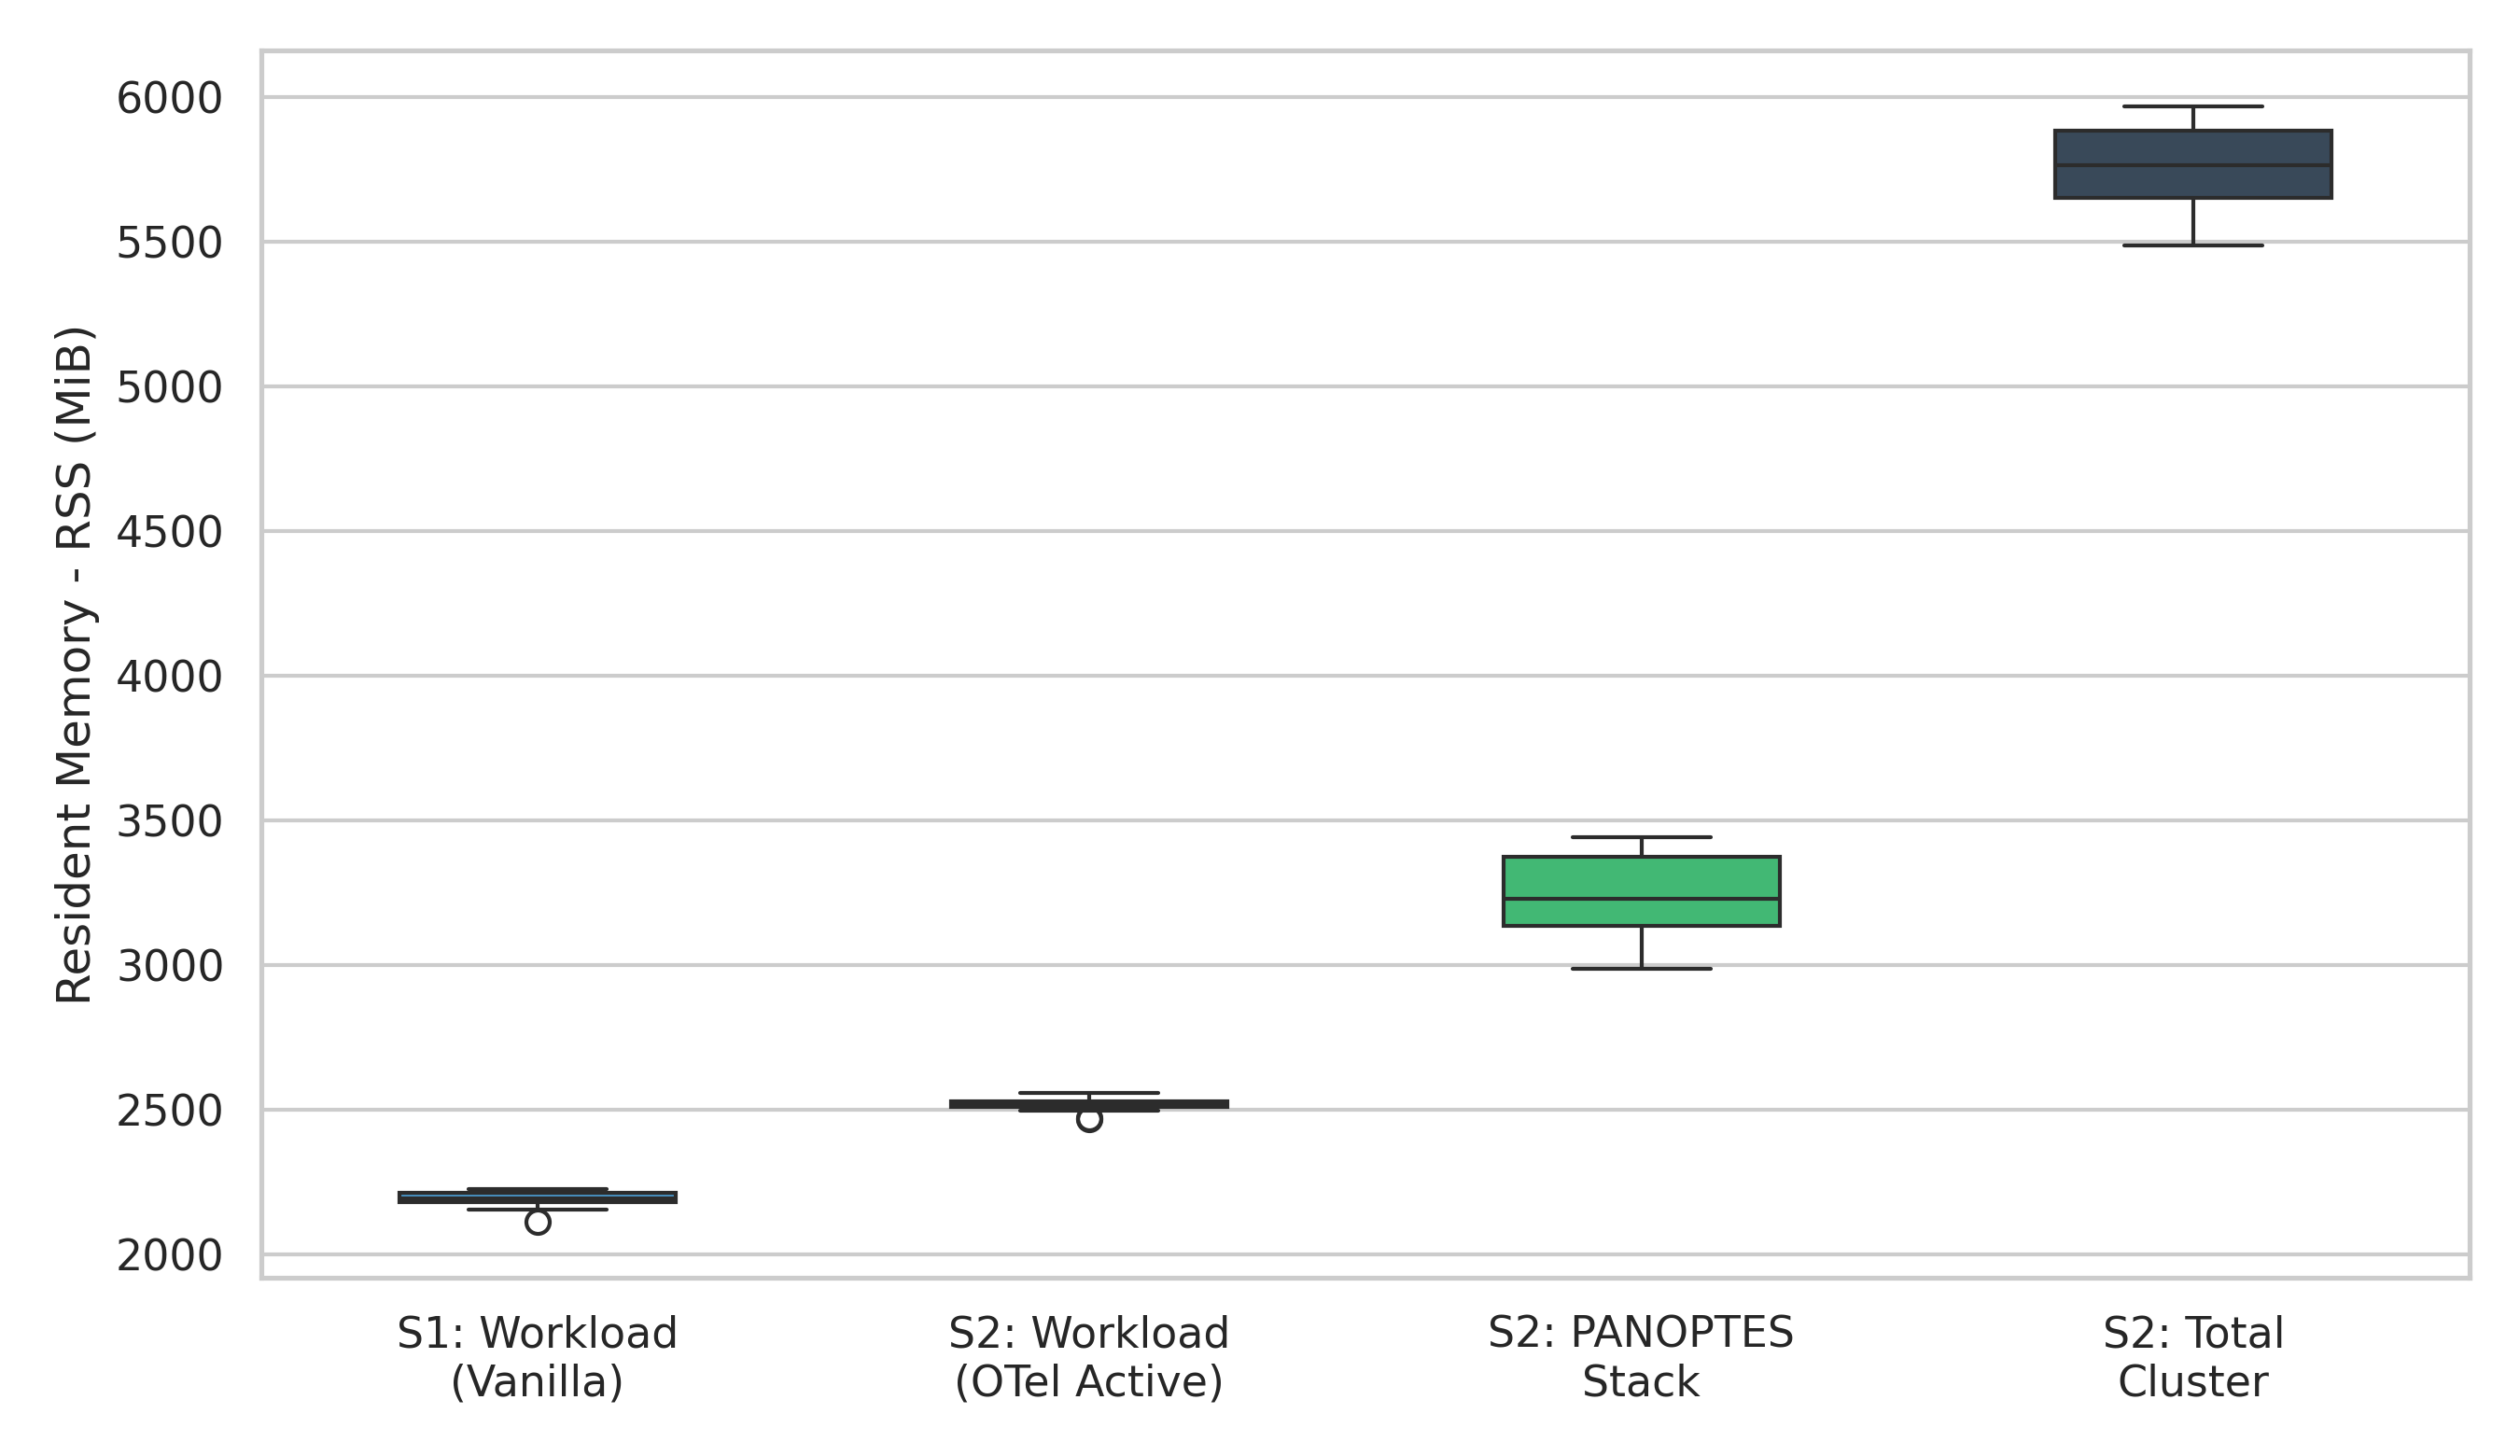
\includegraphics[width=\linewidth, keepaspectratio]{results/scenario2_memory_overhead.png}
    \end{column}
  \end{columns}
\end{frame}

\begin{frame}{Hipótese $H_{1,1}$: Redução Massiva de Latência ($MTTDiag$)}
  \begin{columns}[T]
    \begin{column}{0.55\textwidth}
      \begin{block}{Comparativo Estatístico de $MTTDiag$}
        \scriptsize
        \begin{tabular}{l c c c}
          \toprule
          \textbf{Métrica} & \textbf{Vanilla (S3)} & \textbf{PANOPTES (S4b)} & \textbf{Redução} \\
          \midrule
          \textbf{Mediana} & $300.00\,\text{s}$ & $\mathbf{17.27\,\text{s}}$ & $\mathbf{-94.24\%}$ \\
          \textbf{Média} & $242.42\,\text{s}$ & $\mathbf{54.52\,\text{s}}$ & $\mathbf{-77.51\%}$ \\
          \bottomrule
        \end{tabular}
      \end{block}
      \vspace{-1ex}
      \begin{alertblock}{Testes Estatísticos de Hipótese}
        \scriptsize
        \begin{itemize}
          \item \textbf{Mann-Whitney $U$:} $U = 138.0, \; \mathbf{p = 4.55 \times 10^{-6}}$
          \item \textbf{Wilcoxon Pareado:} $W = 0.0, \; \mathbf{p = 3.06 \times 10^{-5}}$
          \item \textbf{Tamanho de Efeito Vargha-Delaney:} $\mathbf{\hat{A}_{12} = 0.8167}$ (\textit{Large})
        \end{itemize}
      \end{alertblock}
    \end{column}
    
    \begin{column}{0.43\textwidth}
      \centering
      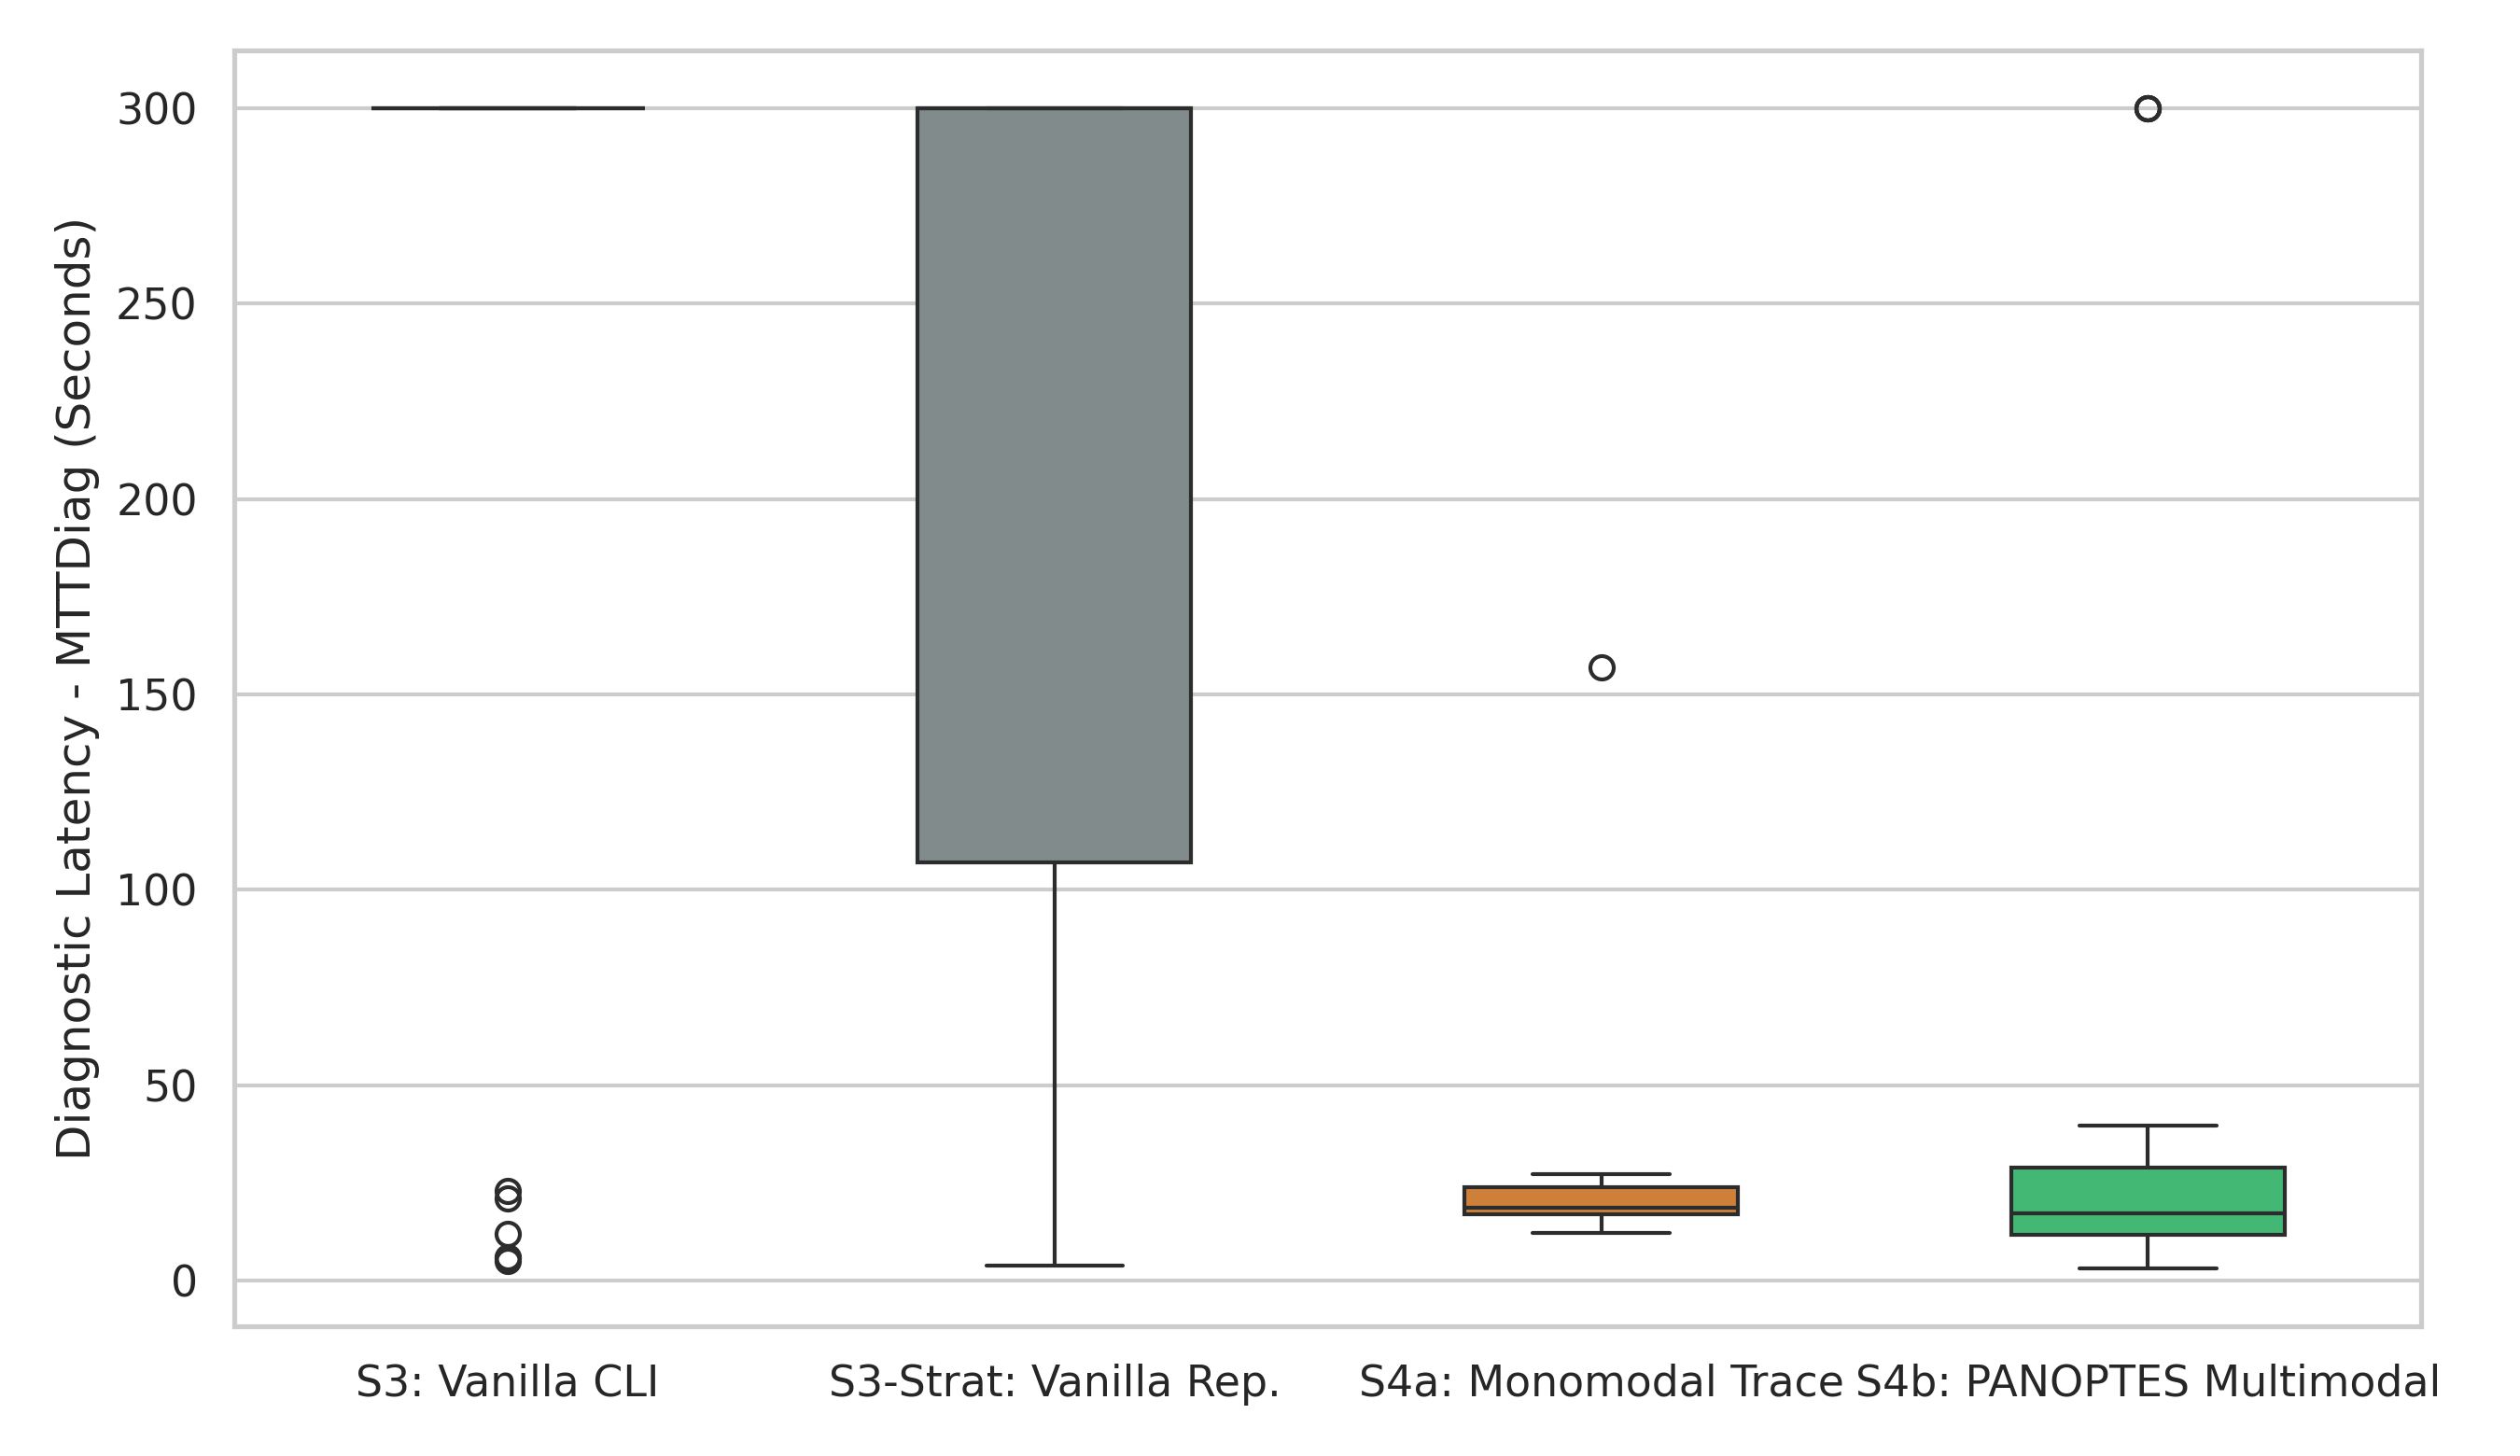
\includegraphics[height=0.62\textheight]{results/final_mttdiag_comparison.png}
    \end{column}
  \end{columns}
  \vspace{0.5ex}
  \centering
  \footnotesize \textbf{Conclusão:} $H_{0,1}$ rejeitada; \textbf{Hipótese $H_{1,1}$ Aceita com Grande Magnitude de Efeito!}
\end{frame}

\begin{frame}{Hipótese $H_{1,2}$: Superioridade em Acurácia Diagnóstica ($Acc$)}
  \begin{columns}[T]
    \begin{column}{0.55\textwidth}
      \begin{block}{Desempenho por Classe de Perturbação}
        \scriptsize
        \begin{tabular}{l c c c}
          \toprule
          \textbf{Classe de Falha} & \textbf{Vanilla} & \textbf{Tracing} & \textbf{PANOPTES} \\
          \midrule
          \texttt{cpu-stress} ($n=10$) & $0.0\%$ & $0.0\%$ & $\mathbf{100.0\%}$ ($10/10$) \\
          \texttt{pod-kill} ($n=10$) & $60.0\%$ & $0.0\%$ & $\mathbf{100.0\%}$ ($10/10$) \\
          \texttt{network-delay} ($n=10$) & $0.0\%$ & $0.0\%$ & $\mathbf{50.0\%}$ ($5/10$) \\
          \midrule
          \textbf{Acurácia Global} & $\mathbf{20.0\%}$ & $\mathbf{0.0\%}$ & $\mathbf{83.33\%}$ ($\mathbf{25/30}$) \\
          \bottomrule
        \end{tabular}
      \end{block}
      \vspace{-1ex}
      \begin{exampleblock}{Testes de Significância e Associação}
        \scriptsize
        \begin{itemize}
          \item \textbf{Fisher's Exact Test:} $\text{Odds Ratio} = \mathbf{20.0}, \; \mathbf{p = 7.74 \times 10^{-7}}$
          \item \textbf{Teste de McNemar (Pareado):} $\chi^2 = 16.05, \; \mathbf{p = 7.83 \times 10^{-5}}$
        \end{itemize}
      \end{exampleblock}
    \end{column}
    
    \begin{column}{0.43\textwidth}
      \centering
      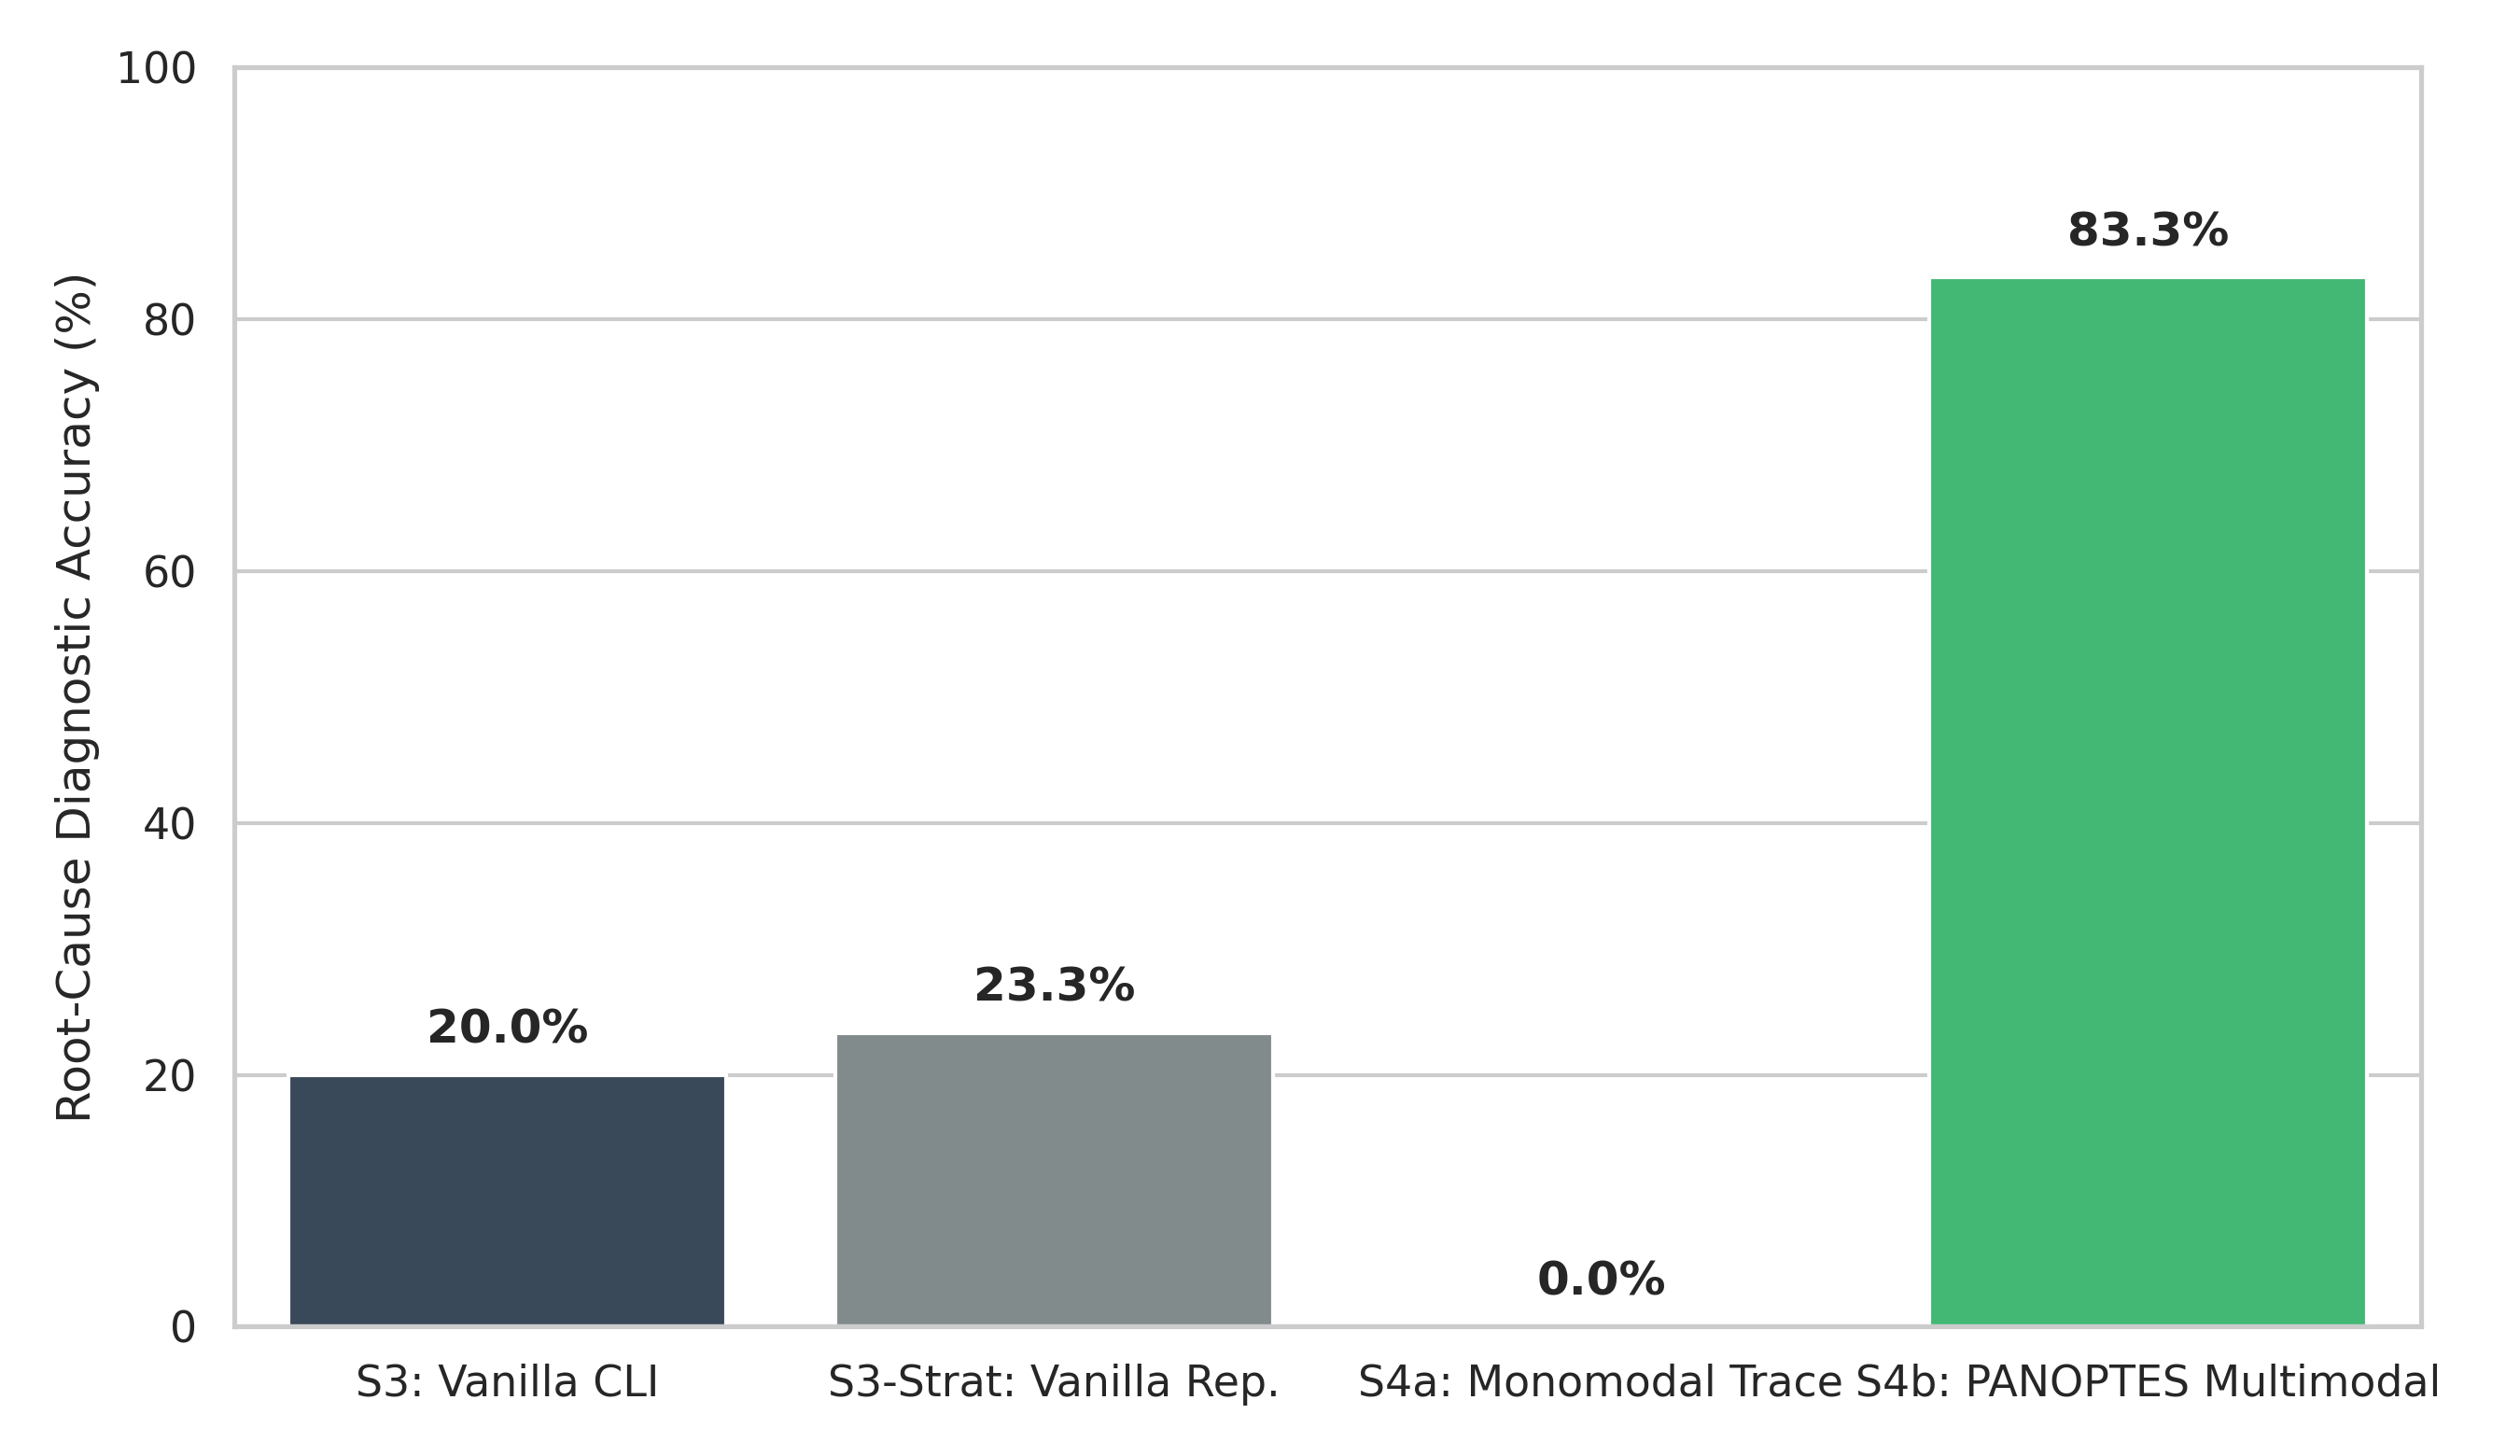
\includegraphics[height=0.62\textheight]{results/final_accuracy_comparison.png}
    \end{column}
  \end{columns}
  \vspace{0.5ex}
  \centering
  \footnotesize \textbf{Conclusão:} $H_{0,2}$ rejeitada; \textbf{Hipótese $H_{1,2}$ Formalmente Aceita!}
\end{frame}

\begin{frame}{Análise de Sobrevivência e Censura (Curvas de Kaplan-Meier)}
  \begin{columns}[T]
    \begin{column}{0.5\textwidth}
      \begin{alertblock}{O Fenômeno da Censura à Direita}
        \begin{itemize}
          \item No Vanilla (S3 e S3-Stratified), \textbf{$73.33\%$ a $80.00\%$} dos ensaios sofreram censura à direita ao esgotar os $300\,\text{s}$ sem resolução.
          \item Falha completa em diagnosticar \texttt{cpu-stress} ($0/11$) e \texttt{network-delay} ($0/10$).
        \end{itemize}
      \end{alertblock}
      
      \begin{exampleblock}{Curva de Sobrevivência PANOPTES}
        \begin{itemize}
          \item Queda acentuada da probabilidade de diagnóstico não-resolvido antes de $30\,\text{s}$;
          \item \textbf{Teste Log-Rank:}
            \begin{equation*}
              \chi^2 = 23.4, \quad \mathbf{p = 1.34 \times 10^{-6}}
            \end{equation*}
        \end{itemize}
      \end{exampleblock}
    \end{column}
    
    \begin{column}{0.5\textwidth}
      \centering
      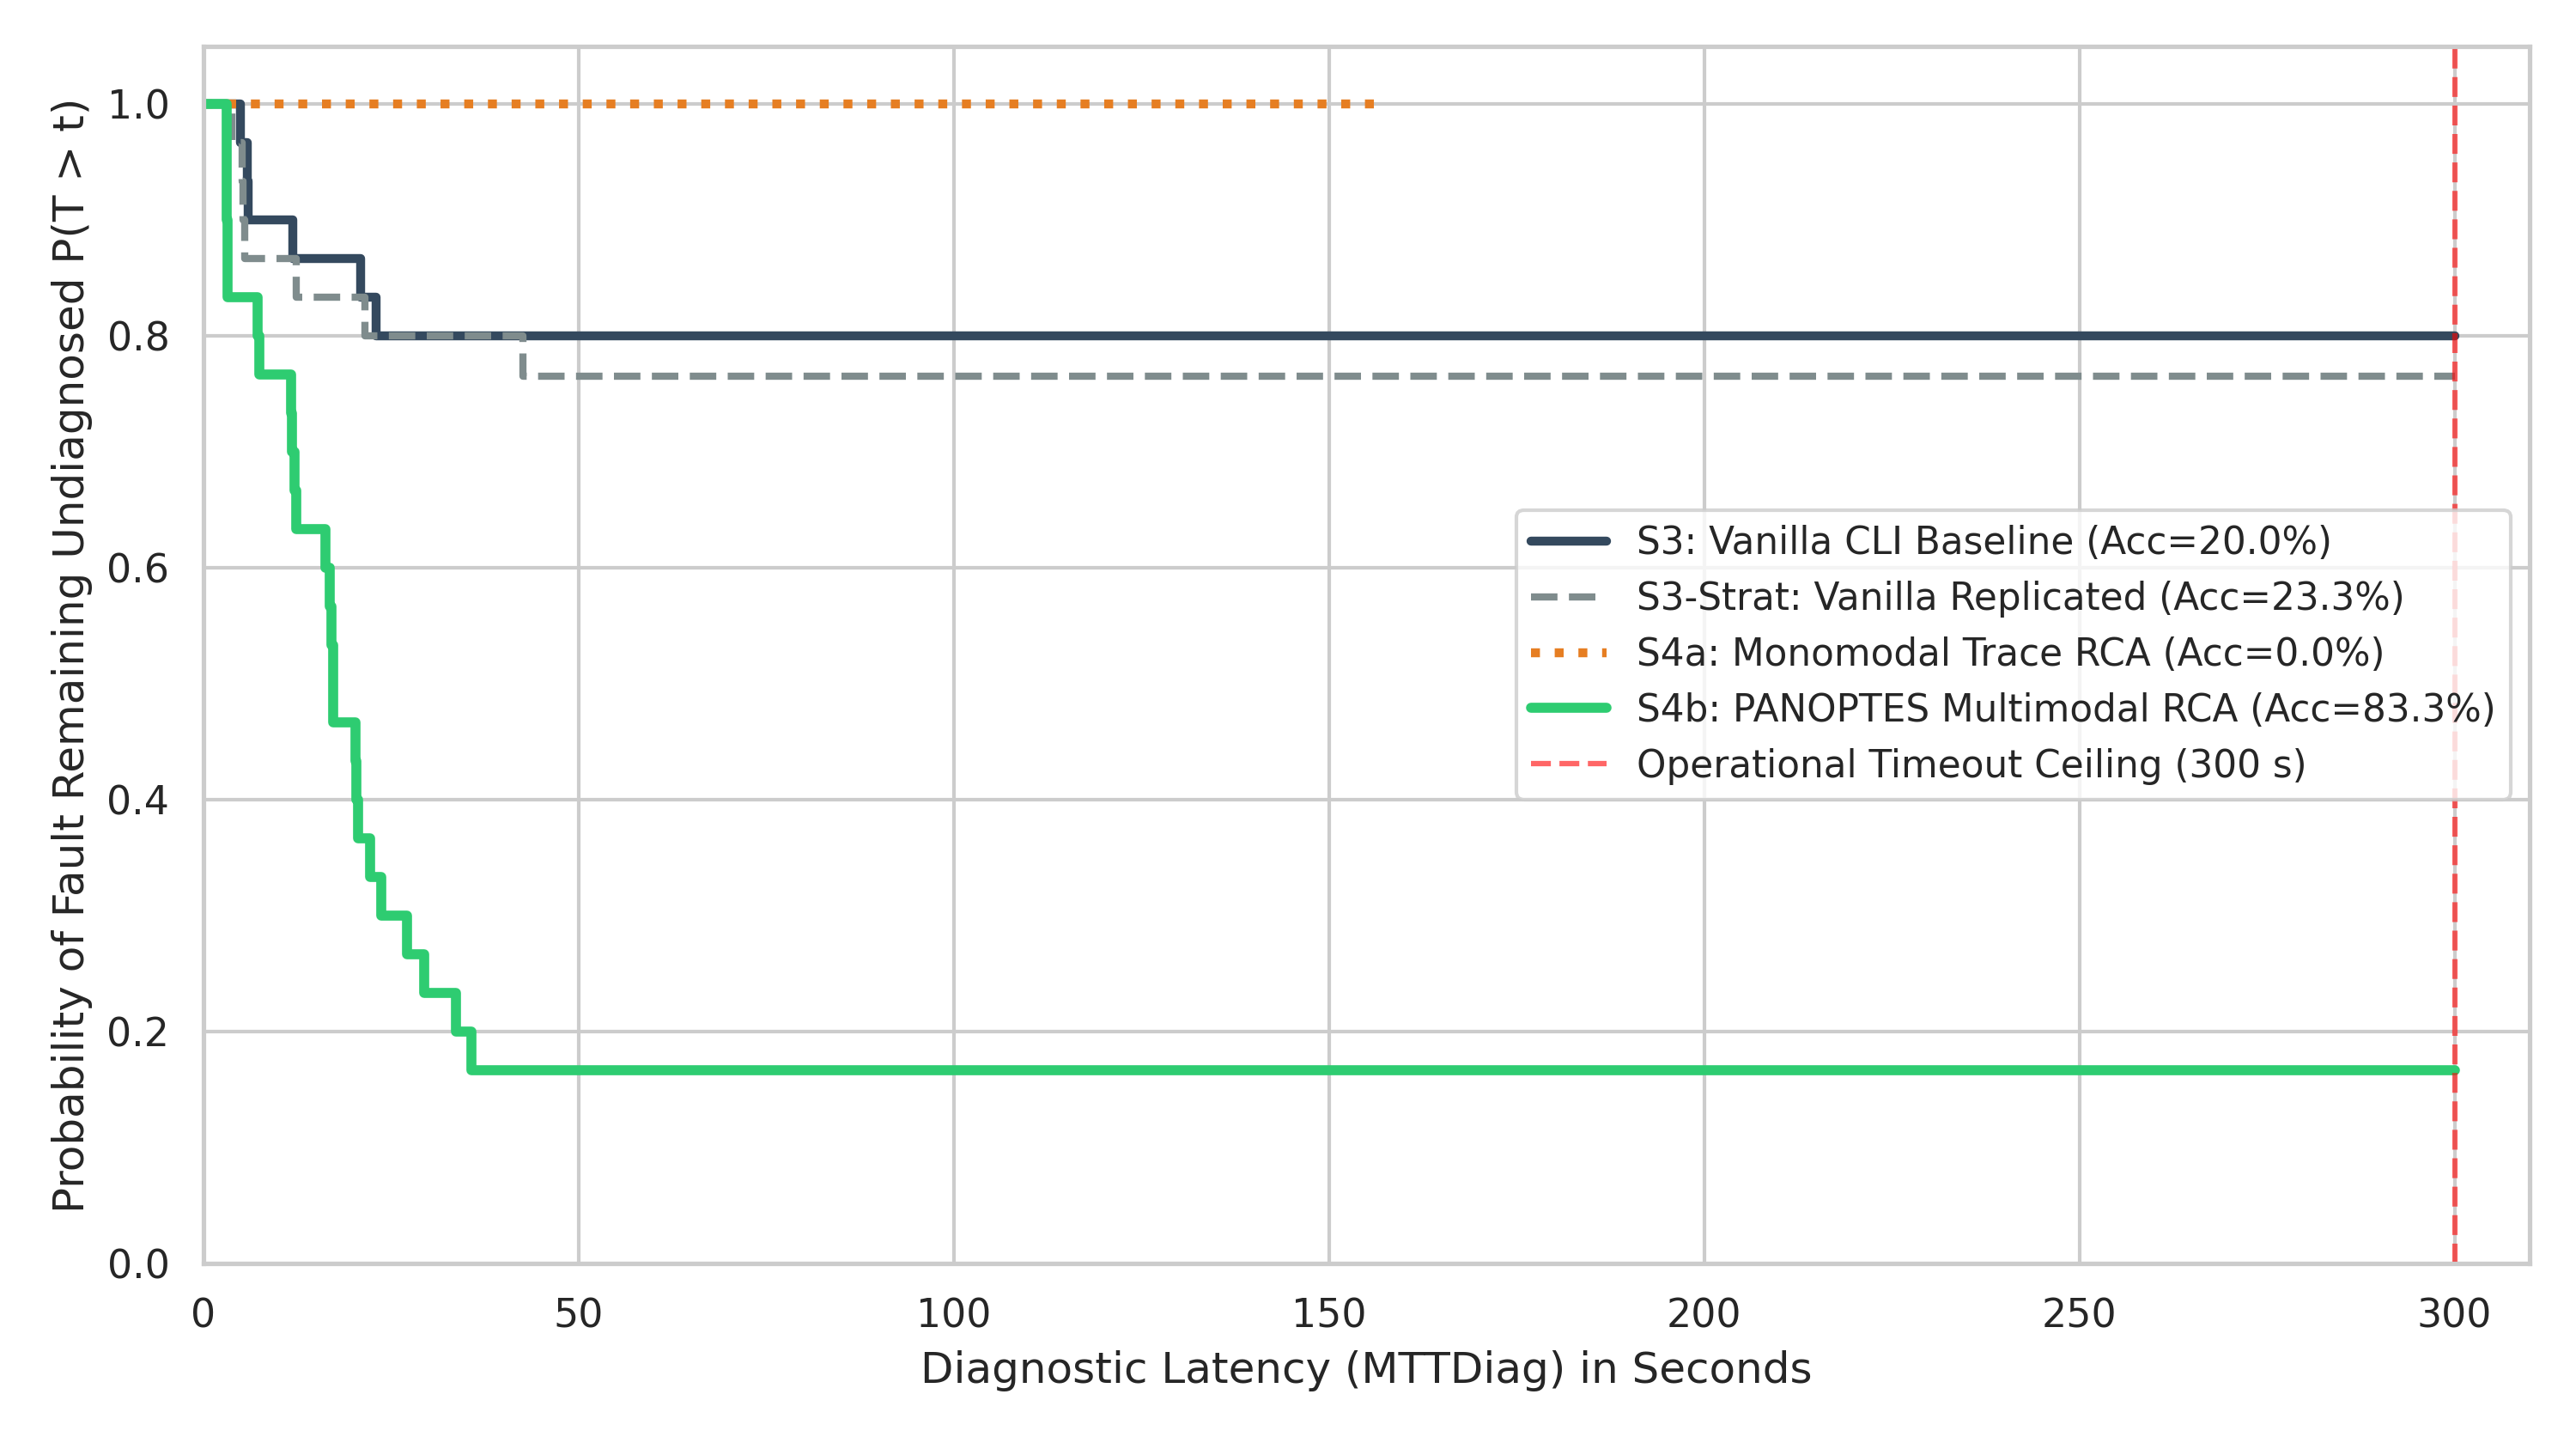
\includegraphics[width=\linewidth]{results/kaplan_meier_survival_curve.png}
    \end{column}
  \end{columns}
\end{frame}

% ==============================================================================
% SECTION 7: DISCUSSION & CONTRIBUTIONS
% ==============================================================================
\section{Discussão, Ameaças à Validade \& Contribuições}

\begin{frame}{Ameaças à Validade \& Estratégias de Mitigação}
  \small
  \begin{tabularx}{\textwidth}{l p{4.5cm} X}
    \toprule
    \textbf{Dimensão} & \textbf{Ameaça Identificada} & \textbf{Mecanismo de Mitigação Implementado} \\
    \midrule
    \textbf{Validade Interna} & Desvio de configuração e interferência entre ensaios (\textit{observer bias}). & Infraestrutura declarativa IaC (\texttt{ConH1}), isolamento de cgroups no K3d (\textbf{ADR-0006}), sanitização de finalizers Chaos Mesh (\textbf{ADR-0004}). \\
    \addlinespace
    \textbf{Validade de Construto} & Vazamento de dados (\textit{data leakage}) no algoritmo de diagnóstico. & Eliminação completa de fallbacks CLI ou leitura de manifestos de injeção (\textbf{ADR-0002}); diagnóstico estritamente via APIs HTTP de telemetria. \\
    \addlinespace
    \textbf{Validade de Conclusão} & Pseudorreplicação temporal e inflação de Erro Tipo I. & Janela de profiling de $16\,\text{s}$ superando os $15\,\text{s}$ do \texttt{metrics-server} (\textbf{ADR-0003}); uso de testes não-paramétricos pareados (Wilcoxon, McNemar). \\
    \addlinespace
    \textbf{Validade Externa} & Representatividade de microsserviços e limitações de laboratório local. & Uso de benchmark de e-commerce representativo da indústria (CNCF Astronomy Shop poliglota); replicação planejada para GCP/GKE em nuvem pública. \\
    \bottomrule
  \end{tabularx}
\end{frame}

\begin{frame}{Síntese das Contribuições da Tese (1/2: Arquitetura \& Artefato)}
  \begin{columns}[T]
    \begin{column}{0.49\textwidth}
      \begin{block}{\large 1. Arquitetura PANOPTES}
        \small
        \textbf{Formalização Teórica \& Princípios de Controle:}
        \begin{itemize}
          \item Estrutura em 4 camadas funcionais desacopladas para orquestradores Kubernetes;
          \item Fundamentação em \textbf{Princípios de Controle} (\texttt{CP1}: Vínculo Causal; \texttt{CP2}: Representação Unificada do Estado);
          \item Definição de \textbf{Heurísticas de Contingência} (\texttt{ConH1}--\texttt{ConH3}) para imunidade ao desvio (\textit{drift}) e contenção do \textit{Efeito Observador}.
        \end{itemize}
      \end{block}
    \end{column}
    
    \begin{column}{0.49\textwidth}
      \begin{block}{\large 2. Artefato Open-Source IaC}
        \small
        \textbf{Instanciação Completa \& Governança:}
        \begin{itemize}
          \item Pilha $100\%$ reproduzível com Infrastructure as Code (Helm charts, playbooks Ansible, scripts de RCA);
          \item Testbed K3d multi-nó com isolamento determinístico de recursos (\texttt{cgroups});
          \item Governança metodológica estrita guiada por 6 Registros de Decisões Arquiteturais (\textbf{ADR-0001} a \textbf{ADR-0006});
          \item Repositório e dados abertos para a comunidade científica.
        \end{itemize}
      \end{block}
    \end{column}
  \end{columns}
\end{frame}

\begin{frame}{Síntese das Contribuições da Tese (2/2: Evidência \& Maturidade)}
  \begin{columns}[T]
    \begin{column}{0.49\textwidth}
      \begin{block}{\large 3. Benchmark Empírico sob Chaos}
        \small
        \textbf{Avaliação Experimental Rigorosa:}
        \begin{itemize}
          \item Primeira base empírica demonstrando o \textbf{colapso do tracing monomodal isolado} sob falhas latentes ($0\%$ de acurácia);
          \item Comprovação da superioridade da \textbf{correlação multimodal} e decomposição de self-time ($\mathbf{83.33\%}$ de acurácia vs. $20\%$ Vanilla);
          \item Redução massiva de $\mathbf{94.24\%}$ na mediana de latência de diagnóstico ($MTTDiag = 17.27\,\text{s}$ vs. $300\,\text{s}$ Vanilla; $p < 10^{-5}$).
        \end{itemize}
      \end{block}
    \end{column}
    
    \begin{column}{0.49\textwidth}
      \begin{block}{\large 4. Modelo de Maturidade (OMM)}
        \small
        \textbf{Formalização de 5 Níveis Evolutivos:}
        \begin{itemize}
          \item Grounded no framework de desenvolvimento de maturidade de Becker et al. (2009);
          \item Preenchimento da \textit{"Lacuna de Validação"} teórica na literatura de engenharia de software (Wendler, 2012);
          \item Instrumento diagnóstico e prescritivo para avaliar e guiar a jornada de observabilidade em orquestradores de contêineres.
        \end{itemize}
      \end{block}
    \end{column}
  \end{columns}
\end{frame}

% ==============================================================================
% SECTION 8: POST-QUALIFICATION ROADMAP & SCHEDULE
% ==============================================================================
\section{Roadmap Pós-Qualificação \& Cronograma}

\begin{frame}{Roadmap de Extensões até a Defesa Final}
  \vspace{-1ex}
  \small
  Visão encadeada em cascata das 4 frentes de evolução técnica e empírica da tese:
  \vspace{0.6ex}

  % Degrau 1
  \noindent\hspace{0.00\textwidth}%
  \begin{minipage}{0.75\textwidth}
    \begin{block}{\scriptsize \textbf{1. Validação Externa em Nuvem Pública (Google Cloud / GKE)}}
      \footnotesize
      Provisionamento gerenciado via Terraform; avaliação sob CNI de nuvem real, volumes persistentes e variabilidade de rede vs. baseline K3d.
    \end{block}
  \end{minipage}

  \vspace{-0.3ex}
  \hspace{0.05\textwidth}\textcolor{cinRed}{$\boldsymbol{\searrow}$}\\[-0.5ex]
  % Degrau 2
  \hspace{0.08\textwidth}%
  \begin{minipage}{0.75\textwidth}
    \begin{exampleblock}{\scriptsize \textbf{2. Refinamento de Detecção Sub-Limiar \& Exemplars ($p95/p99$)}}
      \footnotesize
      Vínculo direto de alta precisão entre histogramas Prometheus e traces do Tempo em rotas esparsas de transação (\texttt{payment}, \texttt{shipping}).
    \end{exampleblock}
  \end{minipage}

  \vspace{-0.3ex}
  \hspace{0.13\textwidth}\textcolor{cinDarkRed}{$\boldsymbol{\searrow}$}\\[-0.5ex]
  % Degrau 3
  \hspace{0.16\textwidth}%
  \begin{minipage}{0.75\textwidth}
    \begin{block}{\scriptsize \textbf{3. Telemetria Zero-Code com eBPF no Kernel (Beyla / Cilium)}}
      \footnotesize
      Sondas no kernel Linux para capturar latências de socket e retransmissões TCP de forma não-invasiva, sem modificar código da aplicação.
    \end{block}
  \end{minipage}

  \vspace{-0.3ex}
  \hspace{0.21\textwidth}\textcolor{cinBlack}{$\boldsymbol{\searrow}$}\\[-0.5ex]
  % Degrau 4
  \hspace{0.24\textwidth}%
  \begin{minipage}{0.75\textwidth}
    \begin{alertblock}{\scriptsize \textbf{4. Fechamento do Ciclo Autonômico de Controle (OMM Nível 5)}}
      \footnotesize
      Acoplamento do motor de RCA a um Kubernetes Operator para executar ações de autocura (\textit{self-healing}) em malha fechada.
    \end{alertblock}
  \end{minipage}
\end{frame}

\begin{frame}{Cronograma até a Defesa Final}
  \scriptsize
  \renewcommand{\arraystretch}{1.15}
  \begin{tabularx}{\textwidth}{l p{3.2cm} X c}
    \toprule
    \textbf{Fase} & \textbf{Período} & \textbf{Atividades Previstas} & \textbf{Entregável} \\
    \midrule
    \textbf{Fase 1} & Meses 1--2 Pós-Quali & Incorporação das recomendações da banca; execução da campanha em nuvem pública (GKE via Terraform). & Testbed GKE \& Dados \\
    \addlinespace
    \textbf{Fase 2} & Mês 3 & Análise comparativa cruzada (K3d local vs. GKE Cloud) e refinamento dos algoritmos de latência. & Capítulo de Resultados \\
    \addlinespace
    \textbf{Fase 3} & Mês 4 & Redação e submissão dos achados empíricos para periódico qualificado (ex.: \textit{JSS}, \textit{IEEE TSC} ou \textit{EMSE}). & Artigo Submetido \\
    \addlinespace
    \textbf{Fase 4} & Meses 5--6 & Revisão final do texto da tese, consolidação do pacote de replicação open-source e \textbf{Defesa Final de Doutorado}. & \textbf{Tese Defendida} \\
    \bottomrule
  \end{tabularx}
\end{frame}

% ------------------------------------------------------------------------------
% Slide: Conclusion & Thank You
% ------------------------------------------------------------------------------
\begin{frame}[plain]
  \begin{center}
    \vspace{2ex}
    {\Huge \textbf{PANOPTES}}\\[1.5ex]
    {\large An Open-Source Reference Architecture for Observability in Kubernetes Ecosystems}\\[3ex]
    
    \textbf{Fagner Fernandes Candido da Silva}\\
    \textit{ffcs@cin.ufpe.br}\\[2.5ex]
    
    \small
    \textbf{Orientador:} Prof. Dr. Vinícius Cardoso Garcia\\
    \textbf{Coorientador:} Prof. Dr. Jackson Raniel Florêncio da Silva\\[2.5ex]
    
    
\includegraphics[height=1.3cm]{HC.png}\\[2ex]
    
    {\large \textbf{Obrigado! / Perguntas \& Discussão}}
  \end{center}
\end{frame}

\end{document}
